% Author: Till Tantau
% Source: The PGF/TikZ manual
\documentclass[a4paper,11pt]{article}
\usepackage[utf8]{inputenc}
\usepackage{listings}
\usepackage{amsmath}    % need for subequations
\usepackage{graphicx}   % need for figures
\usepackage{verbatim}   % useful for program listings
\usepackage{color}      % use if color is used in text
%\usepackage{subfigure}  % use for side-by-side figures
\usepackage{hyperref}   % use for hypertext links, including those to external documents and URLs
\usepackage{url}
\usepackage{float}
\usepackage{todonotes}
\usepackage{tikz}
\usepackage{enumitem}
\usepackage{hyperref}
\usepackage{pdfpages}
\usepackage{caption}
\usepackage{subcaption}
\usepackage{listings}
\usepackage{color}
\usepackage{amsfonts}
\usepackage{latexsym}
\usepackage[T1]{fontenc} % use for allowing < and > in cleartext
\usepackage{fixltx2e}    % use for textsubscript
\usepackage[linesnumbered,boxed,ruled]{algorithm2e}
% \newcommand{\BigO}[1]{\ensuremath{\operatorname{O}\left(#1\right)}}
\newcommand{\BigO}[1]{\ensuremath{\mathop{}\mathopen{}\mathcal{O}\mathopen{}\left(#1\right)}}
\graphicspath{ {./images/} }
\definecolor{mygreen}{rgb}{0,0.6,0}
\definecolor{mygray}{rgb}{0.5,0.5,0.5}
\definecolor{mymauve}{rgb}{0.58,0,0.82}
\lstset{ %
  backgroundcolor=\color{white},   % choose the background color; you must add \usepackage{color} or \usepackage{xcolor}
  basicstyle=\footnotesize,        % the size of the fonts that are used for the code
  breakatwhitespace=false,         % sets if automatic breaks should only happen at whitespace
  breaklines=true,                 % sets automatic line breaking
  captionpos=b,                    % sets the caption-position to bottom
  commentstyle=\color{mygreen},    % comment style
  deletekeywords={...},            % if you want to delete keywords from the given language
  escapeinside={\%*}{*)},          % if you want to add LaTeX within your code
  extendedchars=true,              % lets you use non-ASCII characters; for 8-bits encodings only, does not work with UTF-8
  %frame=single,                    % adds a frame around the code
  keepspaces=true,                 % keeps spaces in text, useful for keeping indentation of code (possibly needs columns=flexible)
  keywordstyle=\color{blue},       % keyword style
  language=Octave,                 % the language of the code
  morekeywords={*,...},            % if you want to add more keywords to the set
  numbers=left,                    % where to put the line-numbers; possible values are (none, left, right)
  numbersep=5pt,                   % how far the line-numbers are from the code
  numberstyle=\tiny\color{mygray}, % the style that is used for the line-numbers
  rulecolor=\color{black},         % if not set, the frame-color may be changed on line-breaks within not-black text (e.g. comments (green here))
  showspaces=false,                % show spaces everywhere adding particular underscores; it overrides 'showstringspaces'
  showstringspaces=false,          % underline spaces within strings only
  showtabs=false,                  % show tabs within strings adding particular underscores
  stepnumber=2,                    % the step between two line-numbers. If it's 1, each line will be numbered
  stringstyle=\color{mymauve},     % string literal style
  tabsize=2,                       % sets default tabsize to 2 spaces
  %title=\lstname                   % show the filename of files included with \lstinputlisting; also try caption instead of title
}

\bibliographystyle{plain}
\begin{document}
\date{March 26th 2014\\ IT University of Copenhagen}
\title{Eye Tracking\\SIGB Spring 2014}

\author{Marcus Gregersen\\
\texttt{mabg@itu.dk}
\and Martin Faartoft\\
\texttt{mlfa@itu.dk}
\and Mads Westi\\
\texttt{mwek@itu.dk}}
\clearpage\maketitle
\thispagestyle{empty}
\setcounter{page}{1}
\newpage

\section{Introduction}
In the following, we will experiment with, and discuss different approaches to detecting major eye features. Figure \ref{fig:eye_features} gives the names of the eye features that are used throughout this report.

\begin{figure}[H]
  \centering
  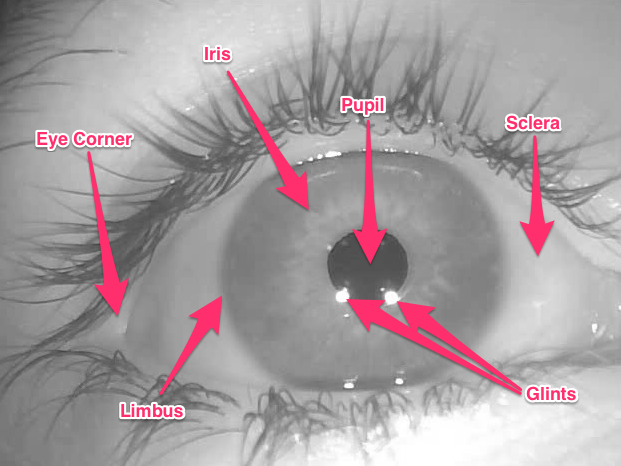
\includegraphics[scale=0.4]{eye_features}
  \caption{Names and positions of major eye features}
  \label{fig:eye_features}
\end{figure}

\section{Pupil Detection}
In this section, we will investigate and compare different techniques for pupil detection.

\subsection{Thresholding}
An obvious first choice of technique, is using a simple threshold to find the pupil, then do connected component (blob) analysis, and finally fit an ellipse on the most promising blobs.

Figure \ref{fig:eye1_threshold_93} shows an example of an image from the 'eye1.avi' sequence and the binary image produced by, using a threshold that blacks out all pixels with intensities above 93. This manages to separate the pupil nicely from the iris.

\begin{figure}[H]
  \centering
  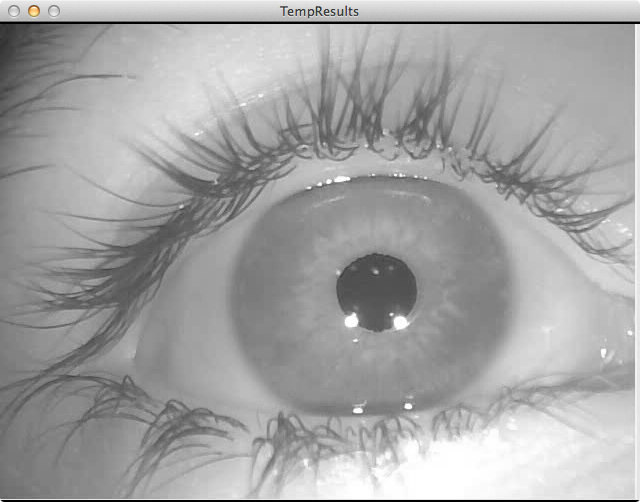
\includegraphics[scale=0.2]{eye1}
  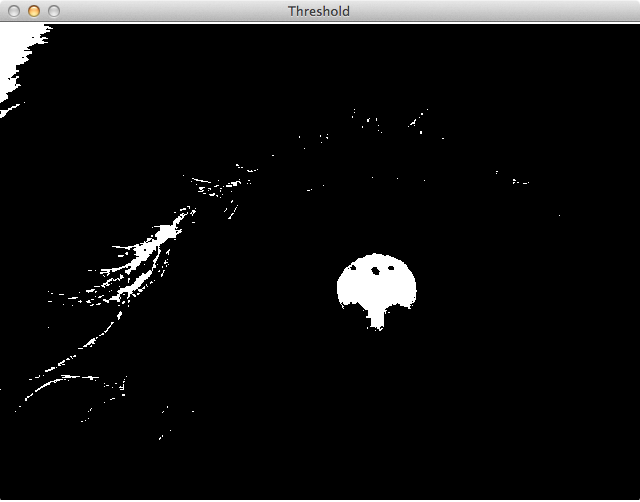
\includegraphics[scale=0.2]{eye1_threshold_93}
  \caption{Thresholding eye1.avi}
  \label{fig:eye1_threshold_93}
\end{figure}

The next step, is to do connected component analysis, and fit an ellipsis through the blobs. As seen in Figure \ref{fig:eye1_unfiltered}, this succesfully detects the pupil, but is extremely prone to false positives.

\begin{figure}[H]
  \centering
  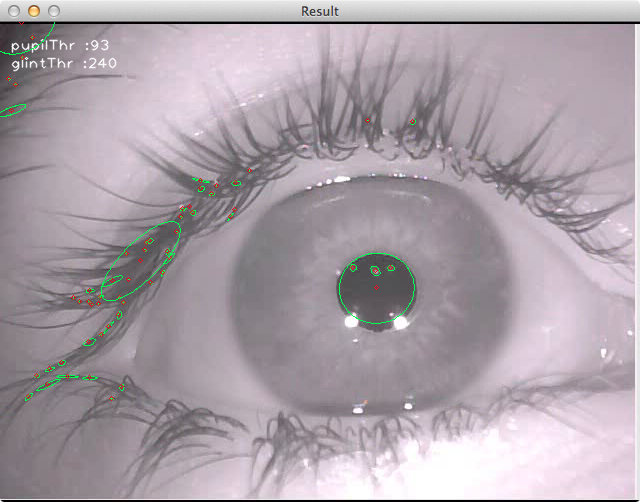
\includegraphics[scale=0.3]{eye1_unfiltered}
  \caption{Fitting ellipses on blobs from eye1.avi (green figures are ellipses fitted through blobs, red dots are the centerpoint of each blob)}
  \label{fig:eye1_unfiltered}
\end{figure}

By experimenting, we find that requiring that the area of the blob lies in the interval $[1000:10000]$, and the extent between $[0.4:1.0]$, we eliminate most false positives on the entire eye1 sequence, while still keeping the true positive.

\paragraph{}
This approach has several problems, however. Note how the true positive on Figure \ref{fig:eye1_unfiltered} fails to follow the bottom of pupil correctly. This is due to the glints obscuring part of the boundary between pupil and iris. It also makes some sweeping assumptions:

\paragraph{The pupil has size at least size 1000}
If the person on the sequence leans back slightly, the pupil will shrink and we will fail to detect it.

\paragraph{A threshold of 93 will cleanly separate pupil from iris}
This is true for eye1.avi, but does not generalize to other sequences. If this approach is to be used across multiple sequences recorded in different lighting conditions, the threshold will have to be adjusted by hand for each one.

This problem can be mitigated somewhat with Histogram Equalization. A threshold of 25 on Histogram Equalized images, fares considerably better across several sequences.

\begin{figure}[H]
  \centering
  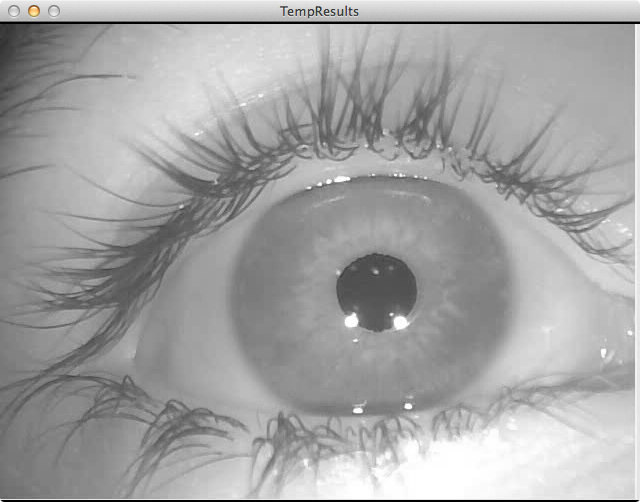
\includegraphics[scale=0.2]{eye1}
  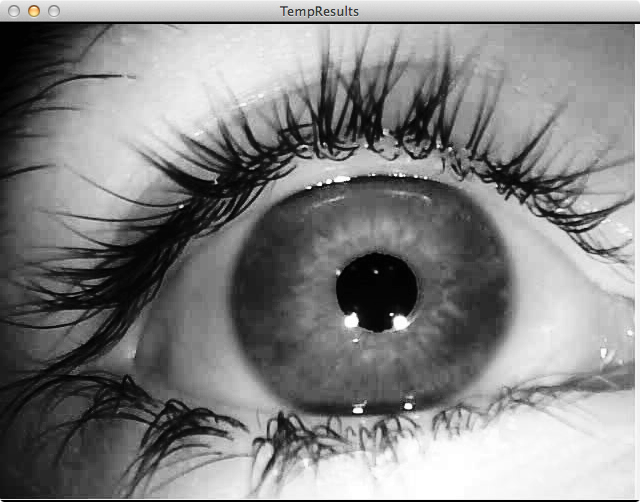
\includegraphics[scale=0.2]{eye1_hist_eq}
  \caption{Eye1 before and after Histogram Equalization}
  \label{fig:eye1_hist_eq}
\end{figure}

\begin{figure}[H]
  \centering
  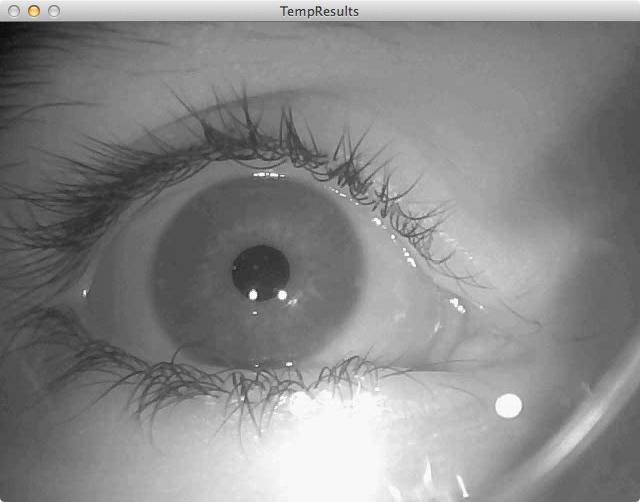
\includegraphics[scale=0.2]{eye3}
  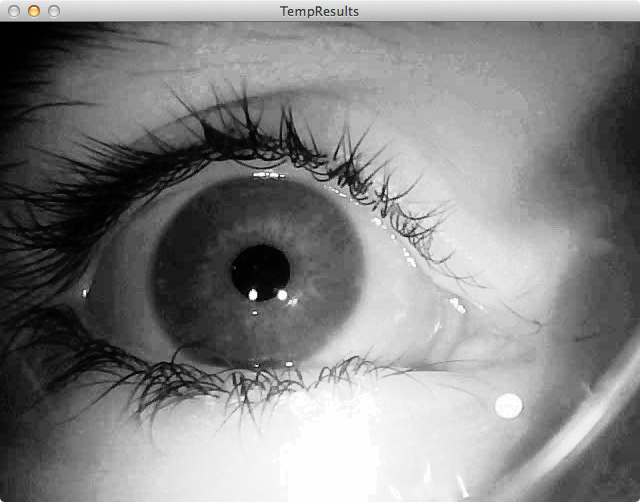
\includegraphics[scale=0.2]{eye3_hist_eq}
  \caption{Eye3 before and after Histogram Equalization}
  \label{fig:eye3_hist_eq}
\end{figure}

\paragraph{Morphology}
Using Morphology, we can improve the detected pupil. The problem with the glints obscuring part of the boundary can be mitigated with the 'closing' operator - used to fill in holes in binary images. Figure \ref{fig:morph} shows binary images before and after applying the closing operator. Notice how the noise inside the pupil is completely removed, and the glints are mostly removed.
A downside to using the closing operation, is that adjacent, sparse structures may merge into something resembling a circle, thereby giving a false positive.

\begin{figure}[H]
  \centering
  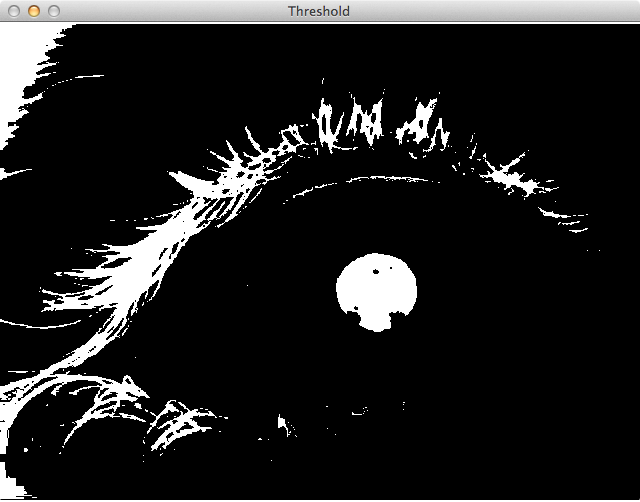
\includegraphics[scale=0.2]{eye1_close_5}
  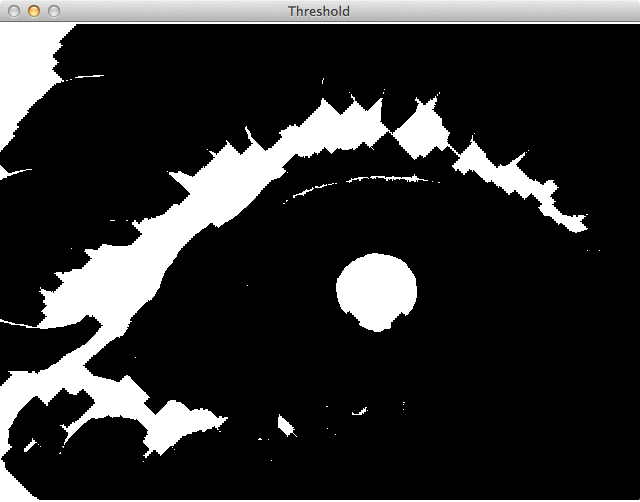
\includegraphics[scale=0.2]{eye1_no_morph}
  \caption{Eye1 before and after Closing (5 iterations, 5x5 CROSS structuring element)}
  \label{fig:morph}
\end{figure}

\paragraph{Tracking} The pupil tracker can be further improved, by using information about the pupil positions from the previous frame. We do it as follows:
\begin{description}
\item[1.]{Search within some threshold distance from each pupil in previous frame}
\item[2.]{One or more pupils were found within the distance, return those}
\item[3.]{No pupils were found within the distance, search the entire image}
\end{description}
Because of the fallback clause in '3', it is very unlikely that the true positive is not detected in each frame. The only case where this approach fails, is if the pupil is obscured for a frame (subject blinking for example), while a false positive is still detected. In that case, the pupil will be improperly detected for as long as the false positive continues to be present.

\subsection{Pupil Detection using k-means}
A method to enhance the BLOB detection of pupil detection is k-means clustering. The method separates the picture in K clusters. Each cluster is a set of pixels, which have values closer to the cluster center, than to other cluster centres -  a cluster center corresponds to mean value of the pixels in the cluster. The value of K is arbitrarily chosen, so that for a sufficiently large number, K the pupil is evaluated as a single separate cluster. If the pupil is a single cluster a binary image can easily be created and BLOB detection would only need to look at the one object. The following figure illustrates how different values of K impacts the segmentation.

\begin{figure}[H]
\centering
\begin{subfigure}{.33\textwidth}
  \centering
  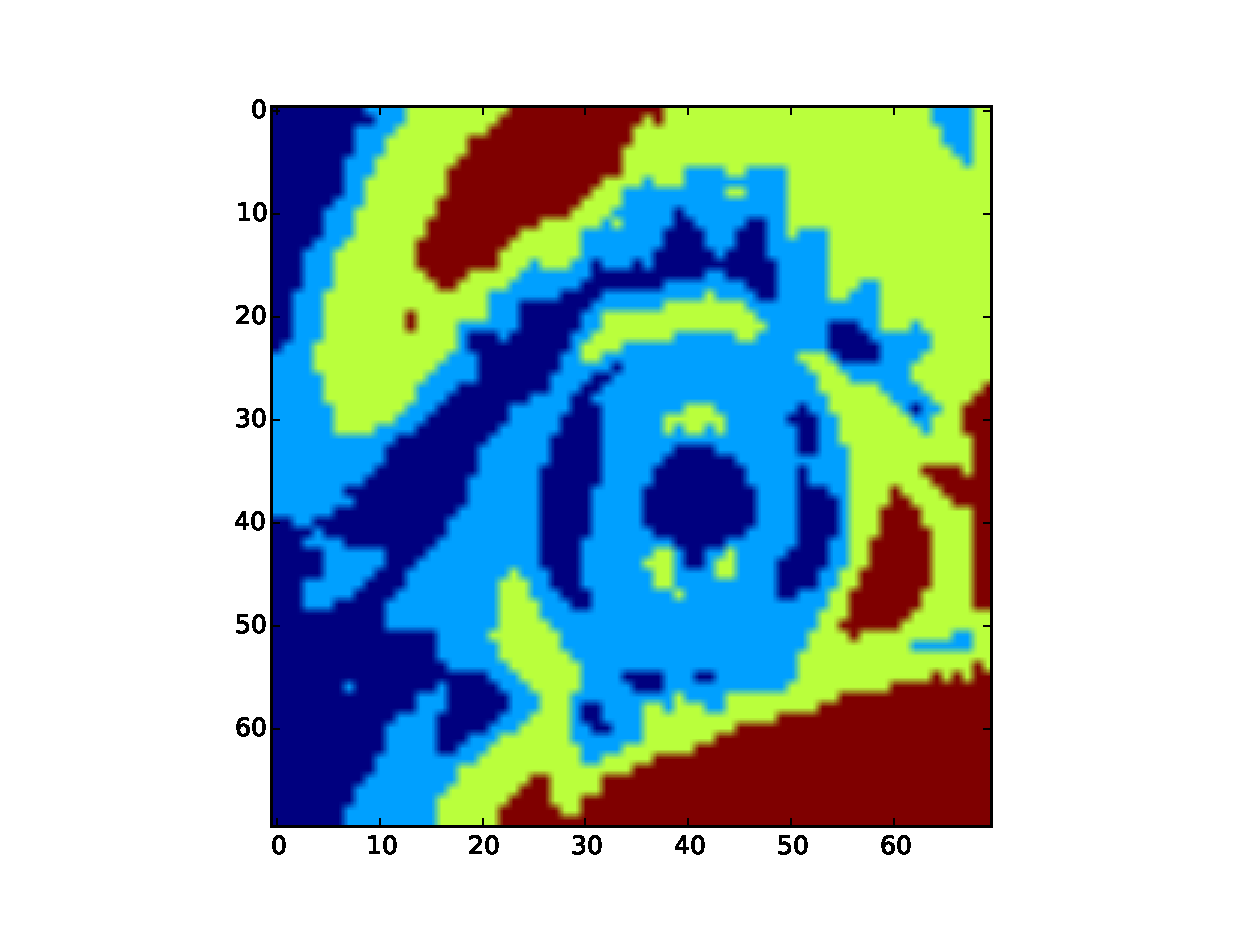
\includegraphics[width=1\linewidth]{kmean_k4_v70}
  \caption{$K=4$}
  \label{fig:kmeans_sub1}
\end{subfigure}%
\begin{subfigure}{.33\textwidth}
  \centering
  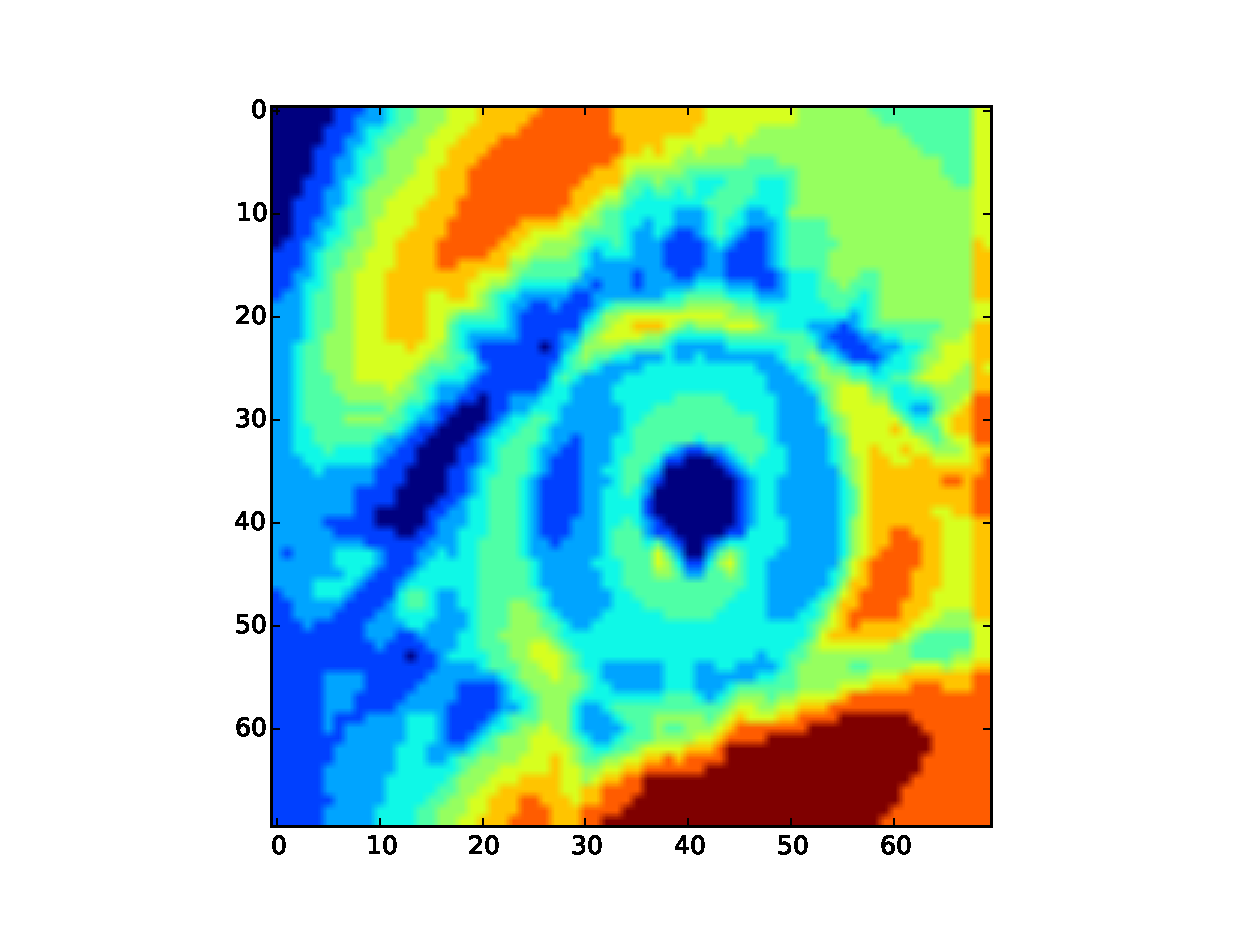
\includegraphics[width=1\linewidth]{kmean_k10_v70}
  \caption{$K=10$}
  \label{fig:kmeans_sub2}
\end{subfigure}
\begin{subfigure}{.33\textwidth}
  \centering
  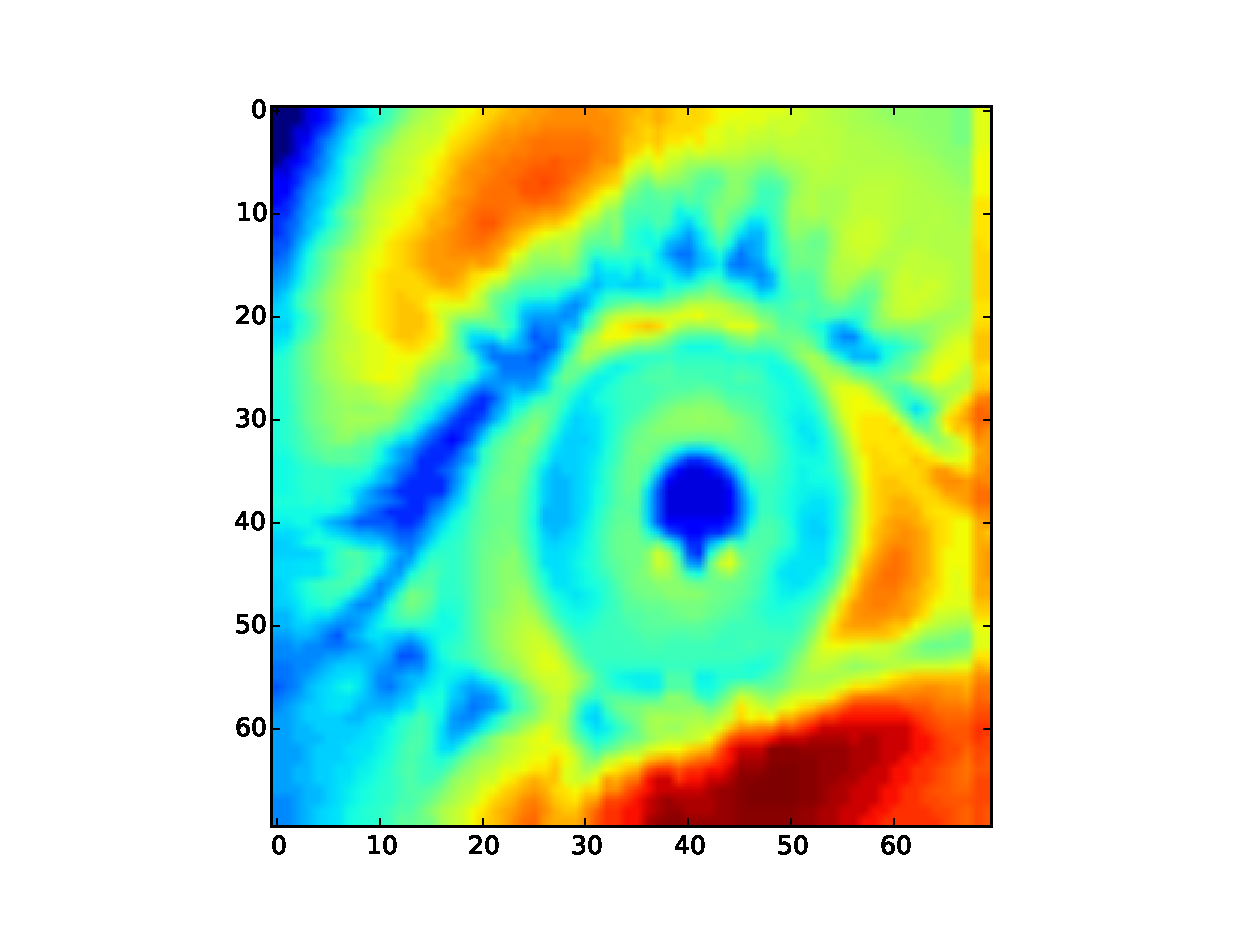
\includegraphics[width=1\linewidth]{kmean_k80_v70}
  \caption{$K=80$}
  \label{fig:kmeans_sub3}
\end{subfigure}
\caption{K-means for different values of $K$}
\label{fig:kmeans_small}
\end{figure}

For performance reasons, the k-means procedure can not be calculated from the original image, the clustering is therefore done on a resized 70x70 pixel image. To reduce the impact of noise, the resized image is filtered with a Gaussian filter. It is clear in figure \ref{fig:kmeans_small} that even for a very high K, the pupil is not a separate cluster, Experiments has revealed that at a K value in the range of 10 to 20 gives a reasonably clustered image, while not having a massive impact on performance.\\

Each pixel in the reduced picture is assigned to a cluster(label), selecting the pixels in the label with the lowest mean value, we can create a binary image, which now can be resized to the original image size. Because the cluster also contains pixels from other regions than the pupil area, the resulting binary image, on which we can do BLOB detection, is not optimal. Figure \ref{fig:kmeans} shows this.

\begin{figure}[H]
\centering
\begin{subfigure}{.5\textwidth}
  \centering
  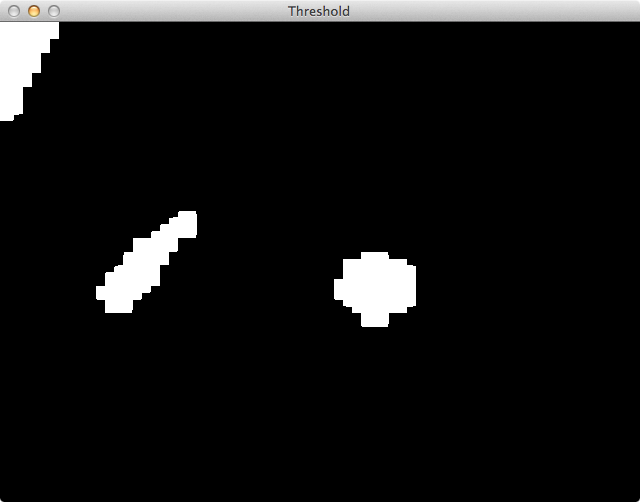
\includegraphics[width=.8\linewidth]{kmean_bin}
  \caption{Binary image}
  \label{fig:kmeans_binary}
\end{subfigure}%
\begin{subfigure}{.5\textwidth}
  \centering
  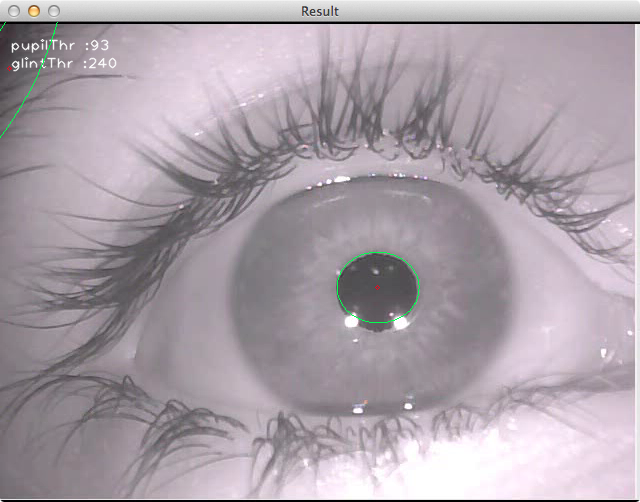
\includegraphics[width=.8\linewidth]{kmean_result}
  \caption{Resulting image}
  \label{fig:kmeans_result}
\end{subfigure}
\caption{Pupil detection using k-means}
\label{fig:kmeans}
\end{figure}

Eyelashes and shadows become a part of the pupil cluster, and much like the issues with morphology, they often become connected components, which makes BLOB detection very difficult.\\

In conclusion the use of k-means did not yield a better result than ordinary thresholding, in many cases the result was actually worse, This is unfortunate because, if the pupil could be found as a single cluster, the amount of evaluation on the BLOB could be reduced and give better scalability on the position of the eye relative to the camera.

\subsection{Pupil Detection using Gradient Magnitude}
So far, we have been looking at the intensity values of the image. This has yielded reasonable approximate results, but is not as robust as we would like. In the following, we investigate what happens if we look at the change in intensity (the image gradient / first derivative), instead of the absolute intensity value at a given point.
The gradients in the X and Y directions, are easily calculated with a Sobel filter. And from these, we can calculate the Gradient Magnitude as: $\sqrt{x^2 + y^2}$ (the Euclidean length of the vector x + y), and the orientation as: $arctan2(y, x)$. Figure \ref{fig:quiver} shows a subsampled cutout of the Gradient image of Eye1, featuring the pupil and glints.

\begin{figure}[H]
  \centering
  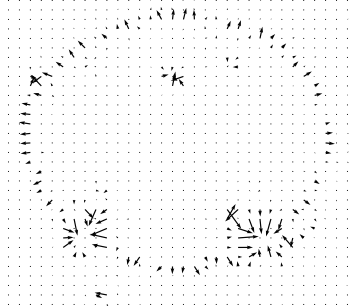
\includegraphics[scale=0.5]{quiver_cutout}
  \caption{Quiver plot of Eye1 gradients (zoomed on pupil area)}
  \label{fig:quiver}
\end{figure}

Note that the pupil boundary is clearly visible on Figure \ref{fig:quiver}. We will attempt to use this information as follows: given an approximate centerpoint and radius for the pupil, scan in a number of directions, $d$ from the centerpoint, find the location of the maximum gradient magnitudes along the line-segments that are described by the centerpoint, a direction from $d$ and the radius. Use this set of points to fit an ellipse, and use that as improved pupil detection.

\begin{figure}[H]
  \centering
  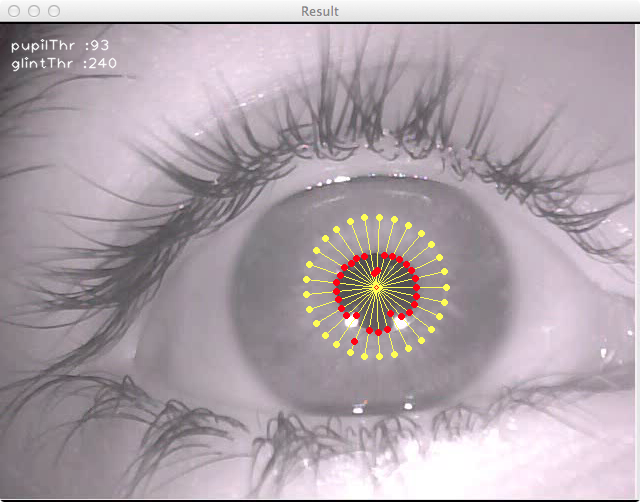
\includegraphics[scale=0.25]{gradient_circle}
  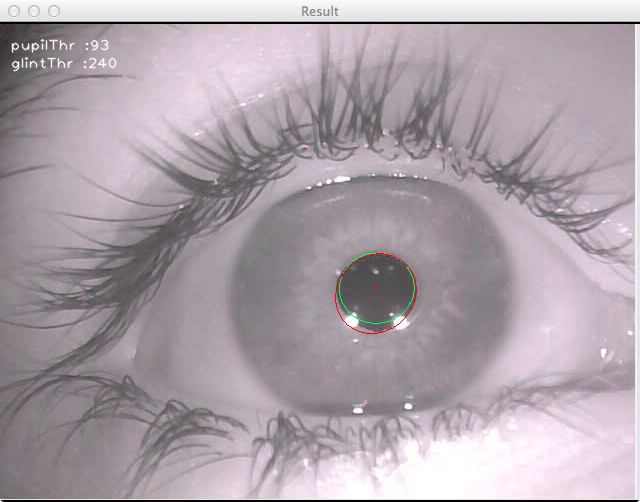
\includegraphics[scale=0.25]{gradient_pupil}
  \caption{Left: Eye1 showing line-segments for gradient magnitude maximization (yellow) and maximum gradient values along the lines (red). Right: Eye1 showing pupil approximation (green), and new pupil detection (red)}
  \label{fig:gradient_circle}
\end{figure}

Figure \ref{fig:gradient_circle}(left) shows the lines considered, and the max gradient points found. Figure \ref{fig:gradient_circle}(right) shows the old and new pupil detections. This approach suffers the same problem as earlier. When the glints obscure part of the boundary, the pupil detection fails to follow the lower boundary. On top of that, there are also issues with noise, notice the red dots inside the top part of the pupil on Figure \ref{fig:gradient_circle}, these are caused by non-system light reflecting off the pupil.

\begin{figure}[H]
  \centering
  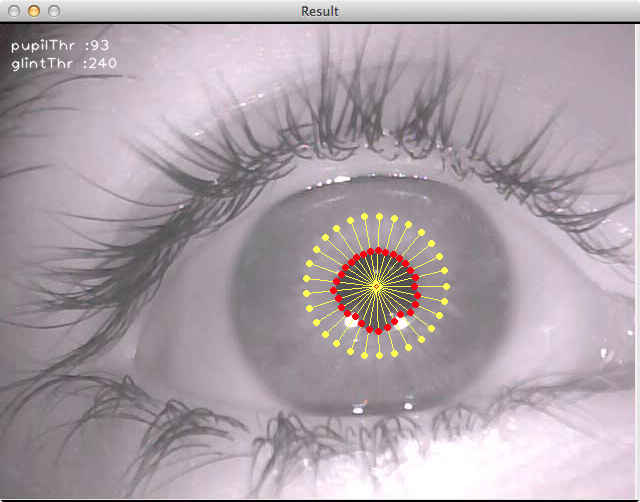
\includegraphics[scale=0.25]{gradient_circle_gaussian_blur}
  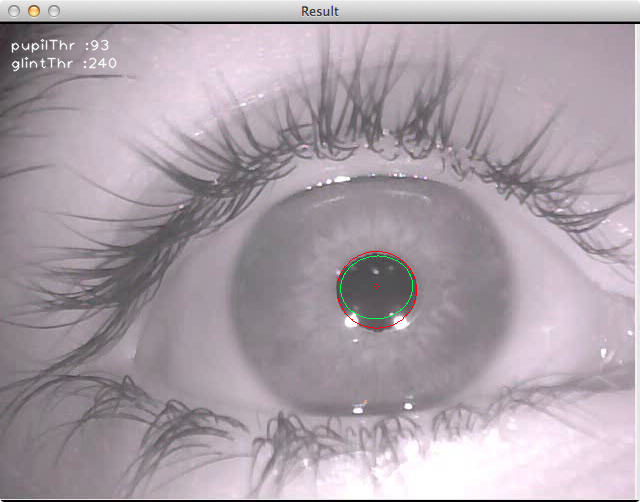
\includegraphics[scale=0.25]{gradient_pupil_gaussian_blur}
  \caption{as Figure \ref{fig:gradient_circle}, but pre-processed with a 9x9 Gaussian Blur}
  \label{fig:gradient_circle_gaussian_blur}
\end{figure}

The noise issues can be drastically reduced with proper pre-processing. Figure \ref{fig:gradient_circle_gaussian_blur} shows much improved results, when blurring the image beforehand.

We experimented with ignoring gradient points where the orientation was too far from the orientation of the circle normal, but did not see any improvements to the pupil detection.

\subsection{Pupil Detection by circular Hough transformation}

In an attempt to make our pupil detection more robust we now investigate the result of applying a
circular Hough transformation on the eye images.

The main challenge is finding the correct parameters for the process. We consider the following parameters:

\begin{description}
  \item[Gauss kernel size] The size of the gaussian kernel that is applied to the image before the Hough transformation

  \item[$\sigma$ - value] the standard deviation value used to construct the gaussian kernel.

  \item[Accumulator threshold] The minimum cumulative vote threshold in which some parameters for a circle are considered.

  \item[Minimum and Maxiumum Radius] The minumum and maximum radius of circles to consider.

\end{description}

The next step is to experimentally find the parameters that yields the best result over all sequences.

\begin{figure}[H]
\centering
\begin{subfigure}{.5\textwidth}
  \centering
  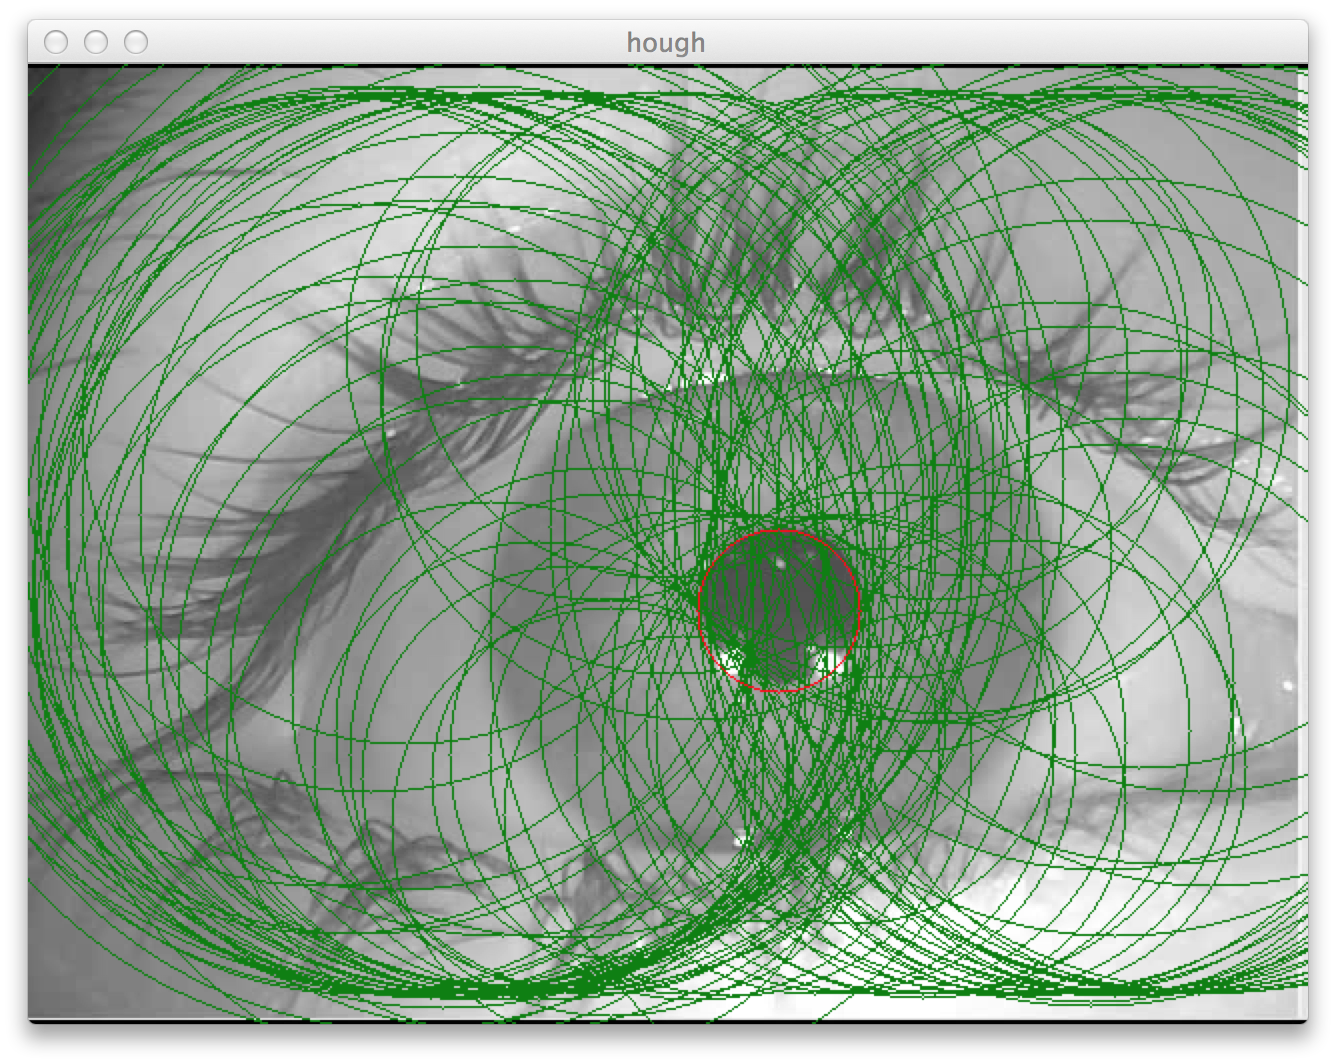
\includegraphics[width=.8\linewidth]{hough100}
  \caption{Accumulator threshold at 100}
  \label{fig:sub1}
\end{subfigure}%
\begin{subfigure}{.5\textwidth}
  \centering
  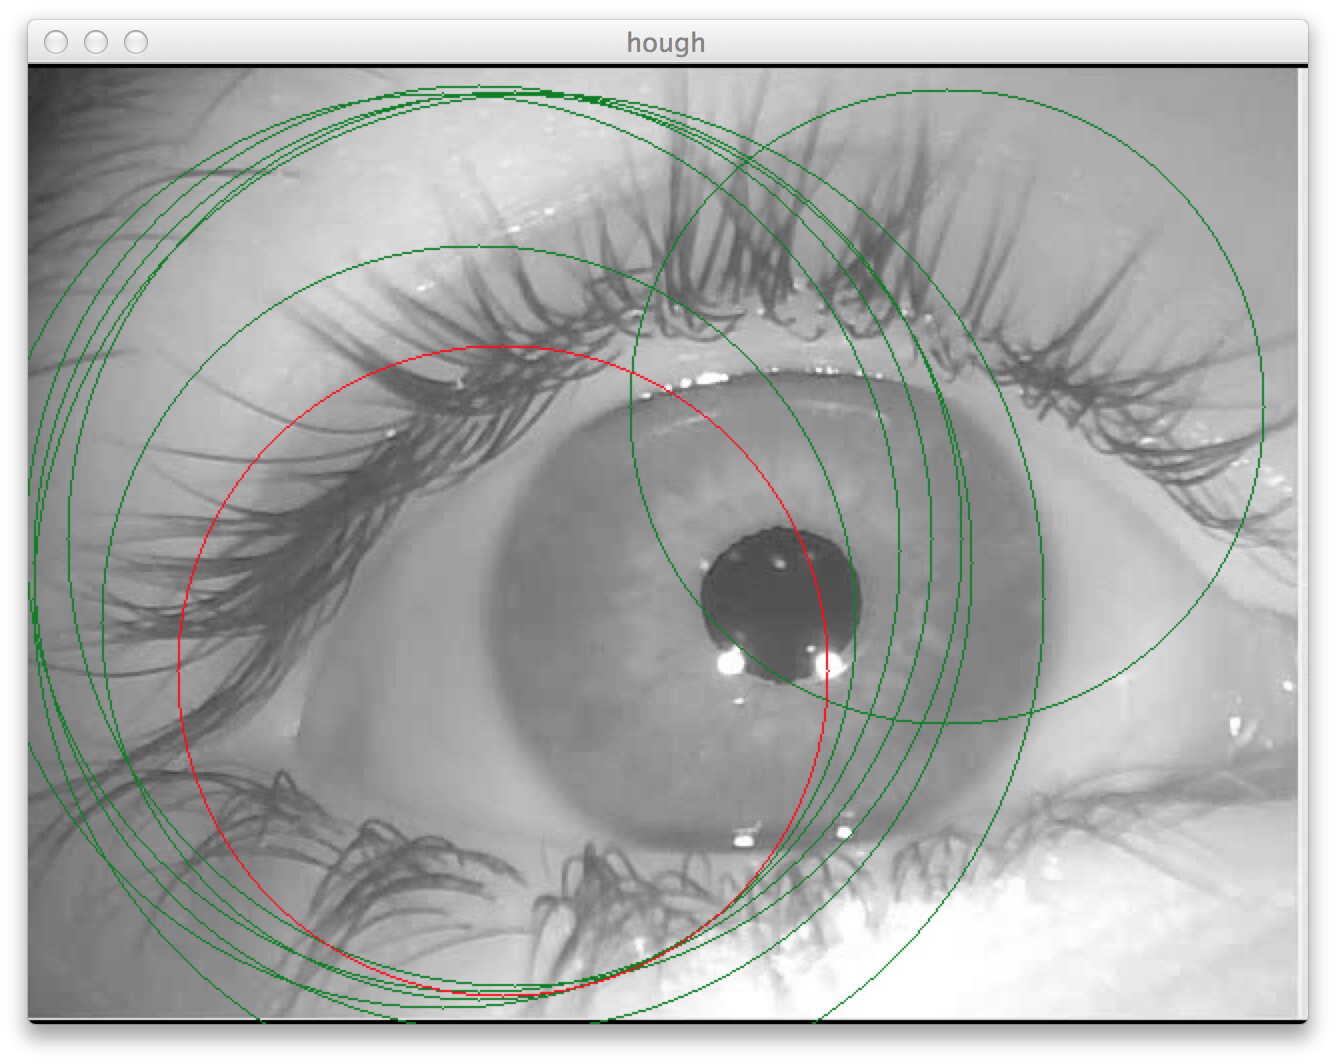
\includegraphics[width=.8\linewidth]{hough150}
  \caption{Accumulator threshold at 150}
  \label{fig:sub2}
\end{subfigure}
\caption{Finding the accumulator threshold values}
\label{fig:test}
\end{figure}

\begin{figure}[H]
\centering
\begin{subfigure}{.5\textwidth}
  \centering
  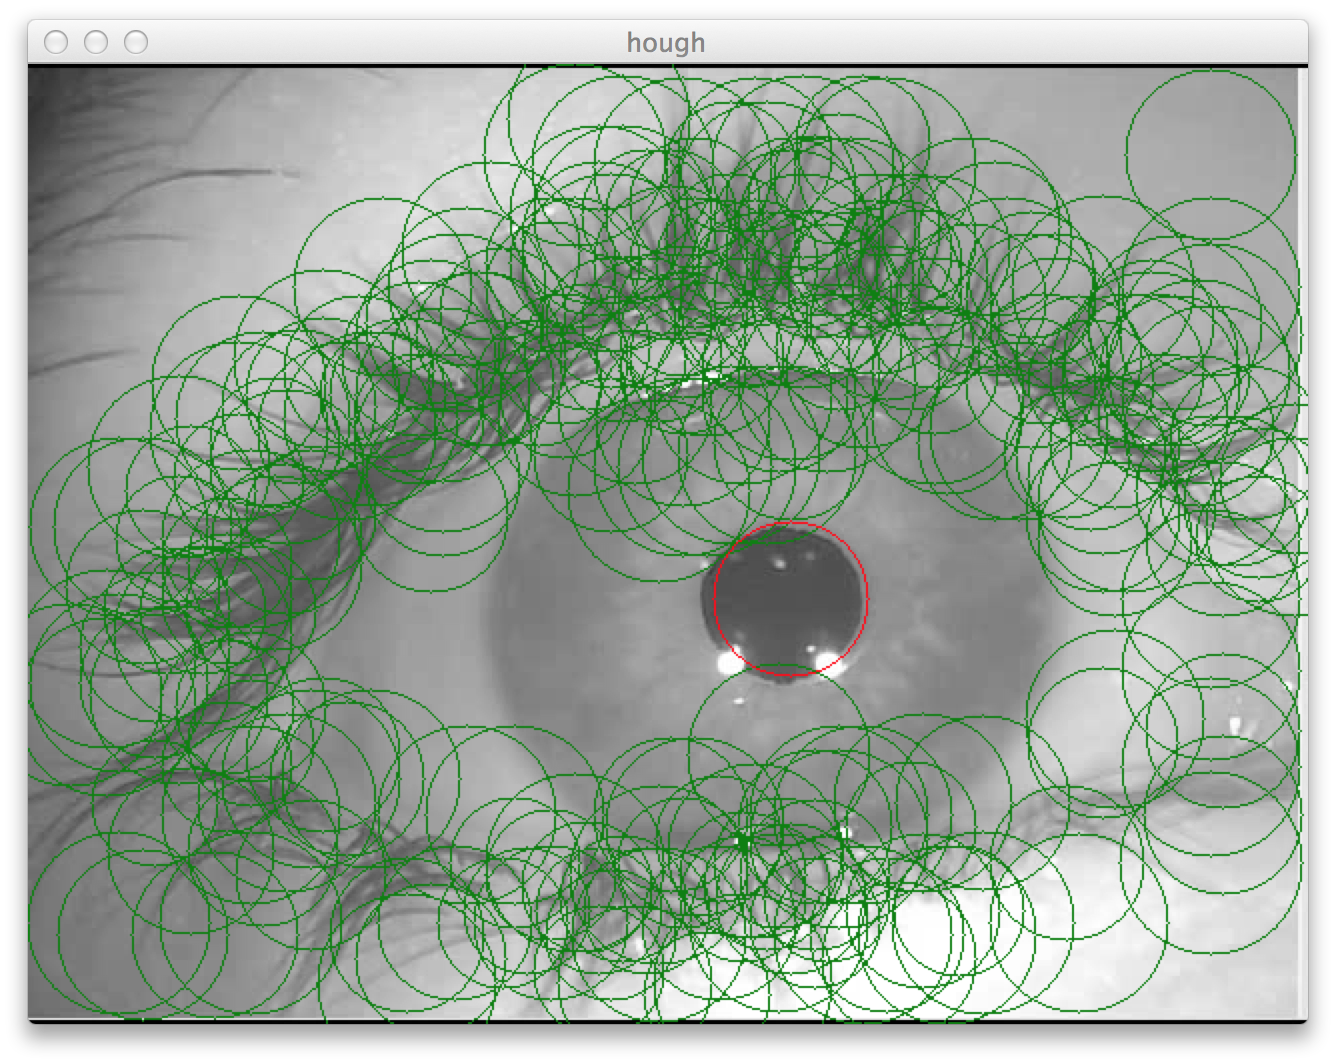
\includegraphics[width=.8\linewidth]{houghk9s9}
  \caption{Size=9, $\sigma$ = 9}
  \label{fig:sub3}
\end{subfigure}%
\begin{subfigure}{.5\textwidth}
  \centering
  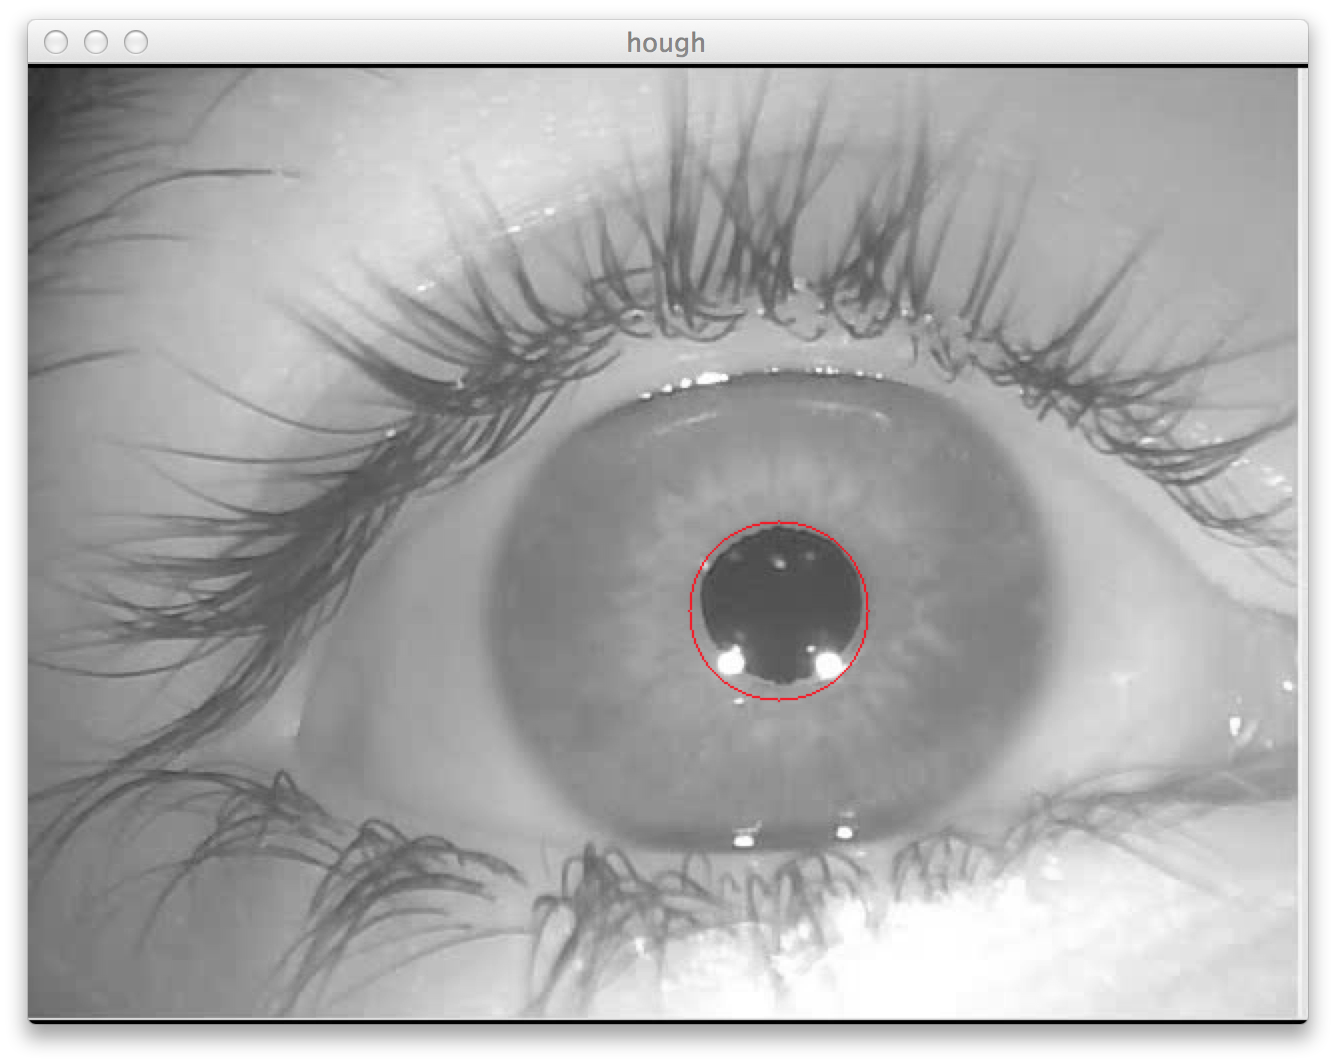
\includegraphics[width=.8\linewidth]{houghk31s9}
  \caption{Size=31, $\sigma$ = 9}
  \label{fig:sub4}
\end{subfigure}
\caption{Preprocessing by smoothing with a gaussian kernel}
\label{fig:test2}
\end{figure}

\paragraph{Discussion}
The circular Hough transformation yields the most robust pupil detection we have been able to produce so far.

The intuition behind this is that in an ideal setting, where the eye for example is not distorted by perspective, the pupil is going to be near-circular, so the process of Hough tranforming and then voting for circles is likely to succeed.

In a non ideal setting, for example in a frame were the eye is seen from the side the pupil is not going to yield the same circular properties, and the process is going to fail.

By preprocessing the image by smooting some of the noise is going to be filtered out. The idea is to choose a kernel that is rougly of the same size as the pupil. In this manner smaller features, such as eye lashes will be smoothed away, but still maintaining the pupil feature.

The drawback of setting a constant size for the gaussian kernel is that is is not scale independent. An ideal kernel in some frame may smoothe away the pupil in some other frame if the had subject moved closer or further away from the camera.

% subsection simplified_hough_transformation (end)

%Hough-transform for ellipsis fitting/detection
%histogram equalization/normalization for making thresholding more robust across sequences
%experiments with morphology

\section{Glint Detection}
In this section, we will investigate and discuss glint detection.

\subsection{Thresholding}
Like pupil detection thresholding seems like an obvious place to start. The methods are almost identical. By first creating a binary image from a threshold value, and then do a BLOB analysis, resulting  in a set of points where glints are present.\\

Figure \ref{fig:glint} shows the glints in ‘eye1.avi’. Because glints are very close to white, a fairly high threshold gives a good result. Furthermore by experimenting we found that, by requiring that the BLOB area lies in the interval $[10:150]$, we exclude a great deal of unwanted glint detections, it is although clear that there is still a good amount of false positives.

\begin{figure}[H]
\centering
\begin{subfigure}{.48\textwidth}
  \centering
  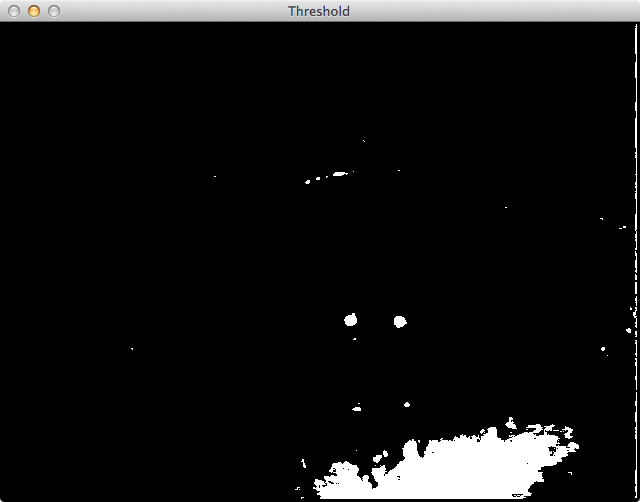
\includegraphics[width=.8\linewidth]{glint_bin}
  \caption{Binary image}
  \label{fig:glint_binary}
\end{subfigure}
\begin{subfigure}{.48\textwidth}
  \centering
  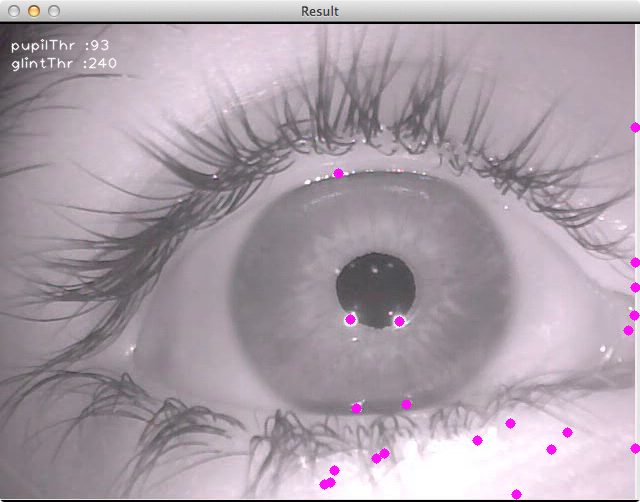
\includegraphics[width=.8\linewidth]{glint_result}
  \caption{Resulting image}
  \label{fig:glint_result}
\end{subfigure}
\caption{Glint detection with threshold of 240}
\label{fig:glint}
\end{figure}

\paragraph{Morphology} To mitigate the false positives, we make use of morphology to remove small “spots” of white by first closing and then opening, we get rid of a lot of unwanted glints, as can be seen in figure \ref{fig:glint_morph}

\begin{figure}[H]
\centering
\begin{subfigure}{.48\textwidth}
  \centering
  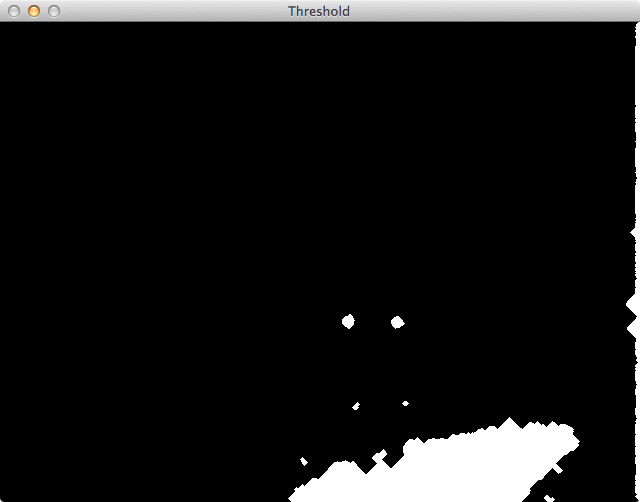
\includegraphics[width=.8\linewidth]{glint_bin_morph}
  \caption{Binary image}
  \label{fig:glint_binary_morph}
\end{subfigure}
\begin{subfigure}{.48\textwidth}
  \centering
  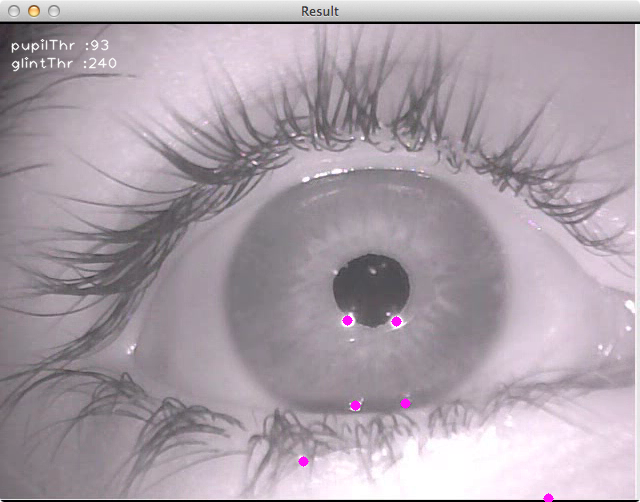
\includegraphics[width=.8\linewidth]{glint_result_morph}
  \caption{Resulting image}
  \label{fig:glint_result_morph_morph}
\end{subfigure}
\caption{Glint detection with threshold of 240 - using morphology}
\label{fig:glint_morph}
\end{figure}

\paragraph{Filter glints using eye features} To further enhance glint detection we have added a function function that excludes glints that have an Euclidian distance from the center of the pupil greater than the largest radius of the elipse representing the pupil. Figure \ref{fig:glint_filtered}

\begin{figure}[H]
\centering
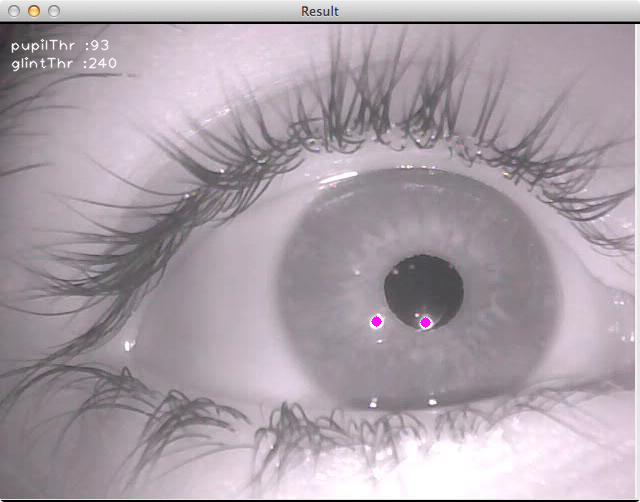
\includegraphics[width=.6\linewidth]{glint_filtered}
\caption{Glint detection with threshold of 240 - using morphology and filter}
\label{fig:glint_filtered}
\end{figure}

\paragraph{Discussion} The method works very well, but fail when more than one pupil is detected, in other words the stability of glint detection is dependent the quality of the pupil detection.

%current:
%threshold->morphology->contour detection->contour filtering->distance from pupil center

%what assumptions do we make?
%how does it perform, when does it work, what causes it to fail
%test on own sequence

%improvements:
%Laplacian?
%hist equal?

\section{Eye Corner Detection}
We detect eye corners simply by template matching. We use template matching by normalized cross-correlation, which is invariant to lighting and exposure conditions, at the expense of performance. Because of the large changes in intensities in the different sequences, we find this to be the preferred method.

\paragraph{Examples}
\begin{figure}[H]
\centering
\begin{subfigure}{.32\textwidth}
  \centering
  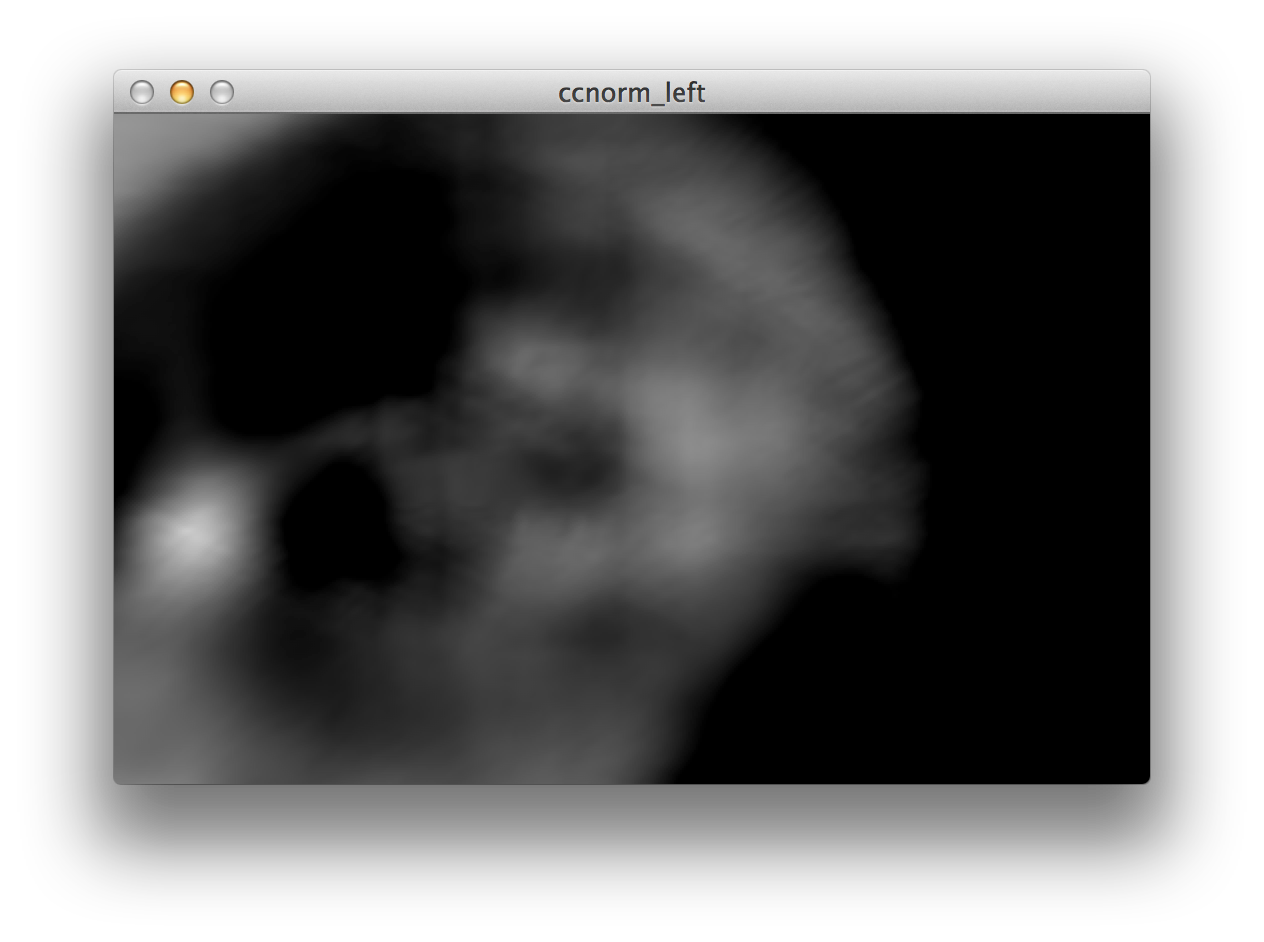
\includegraphics[width=.8\linewidth]{templatematch}
  \caption{image}
  \label{fig:templatemathing1}
\end{subfigure}
\begin{subfigure}{.32\textwidth}
  \centering
  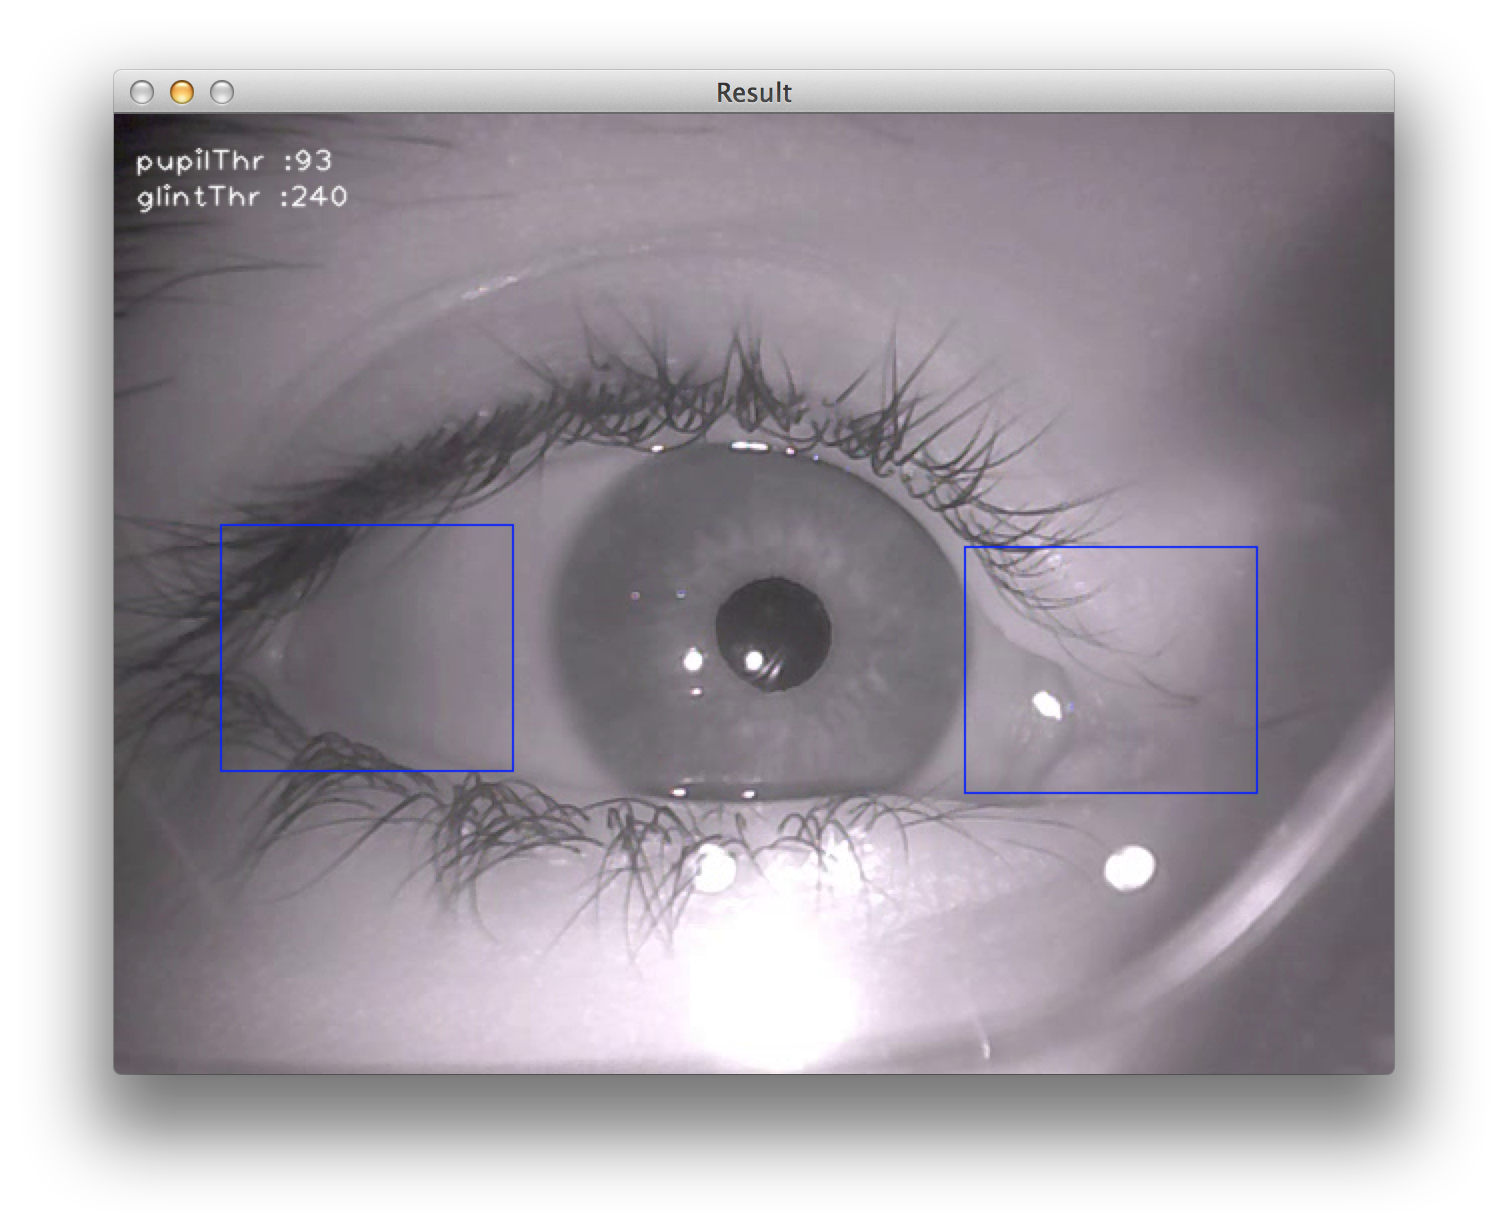
\includegraphics[width=.8\linewidth]{templatematched}
  \caption{A good template match of both the left and right patch}
  \label{fig:templatemathing2}
\end{subfigure}
\begin{subfigure}{.32\textwidth}
  \centering
  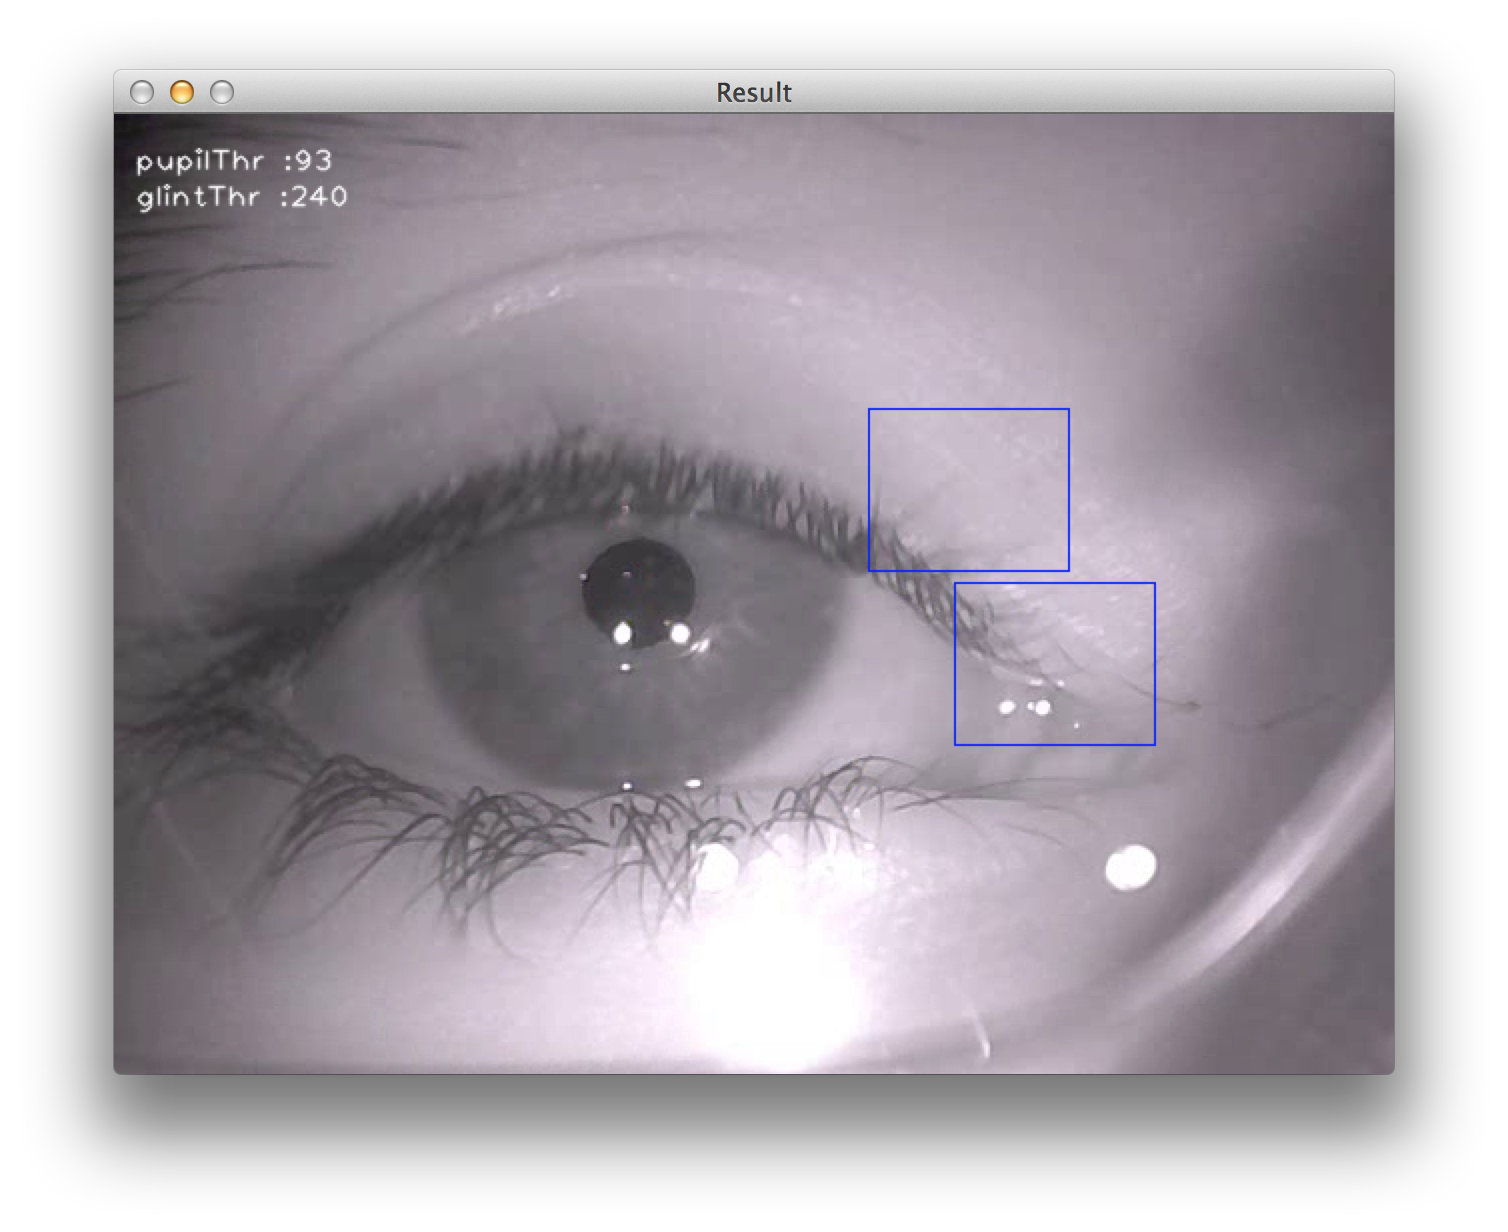
\includegraphics[width=.8\linewidth]{templateproblem}
  \caption{A bad match of the left template}
  \label{fig:templatemathing23}
\end{subfigure}
\caption{Template Matching }
\label{fig:templatemathing}
\end{figure}

The technique works best in a stable environment. Thus if the test subject moves his/her head on any of the 3 axis, or closer/further away from the camera, the chosen template will of course produce a lower result at the position of the actual eye corner.

The changes in scale can be mitigated by using an image pyramid, i.e. convolving the template with multiple versions of a downsampled or upscaled version of the input frame.

Changes in rotation can be mitigated in a similar manner by rotating the template in a number of steps around its own axis.

Changes in perspective, i.e if the person turns his/her head, could possibly be mitigated by transforming the image by a homography.

The methods can be combined to detect a change in both scale and rotation. A problem with these techniques is that they introduce some computational complexity.



\section{Iris / Limbus Detection}
\subsection{Iris detection using thresholding}
We experimented with simple thresholding, to detect the shape and position of the iris. What we found, was that it will work under ideal circumstances, but is extremely brittle with regards to chosen threshold and system lighting. Furthermore, because the iris intensities lies in the middle range (with glints being very bright, and pupil being very dark), many false positives were being picked up in the skin-tone range. This experiment yielded no usable results, and are not discussed further.
\subsection{Hough Transformation with position prior}
If we assume that we are somehow able to detect the pupil in a robust way, we can use this position as input to a circular Hough tranformation.

In this way the Hough tranformation will be one dimensional since the only free variable is the radius of the circle.

The procedure is then to iterate over the circles in a range between some minimum and maximum radius with some step size. We then discretize the periphery of the circle and iterate over this discretization. We then increment the value of the current radius, in a parametric accumulator table, if the corresponding point in the Canny edge image is larger than zero.

The radius with the highest value in the accumulator table is thus the circle that yields the best fit.

\paragraph{Examples}
\label{par:examples}
\begin{figure}[H]
\centering
\begin{subfigure}{.48\textwidth}
  \centering
  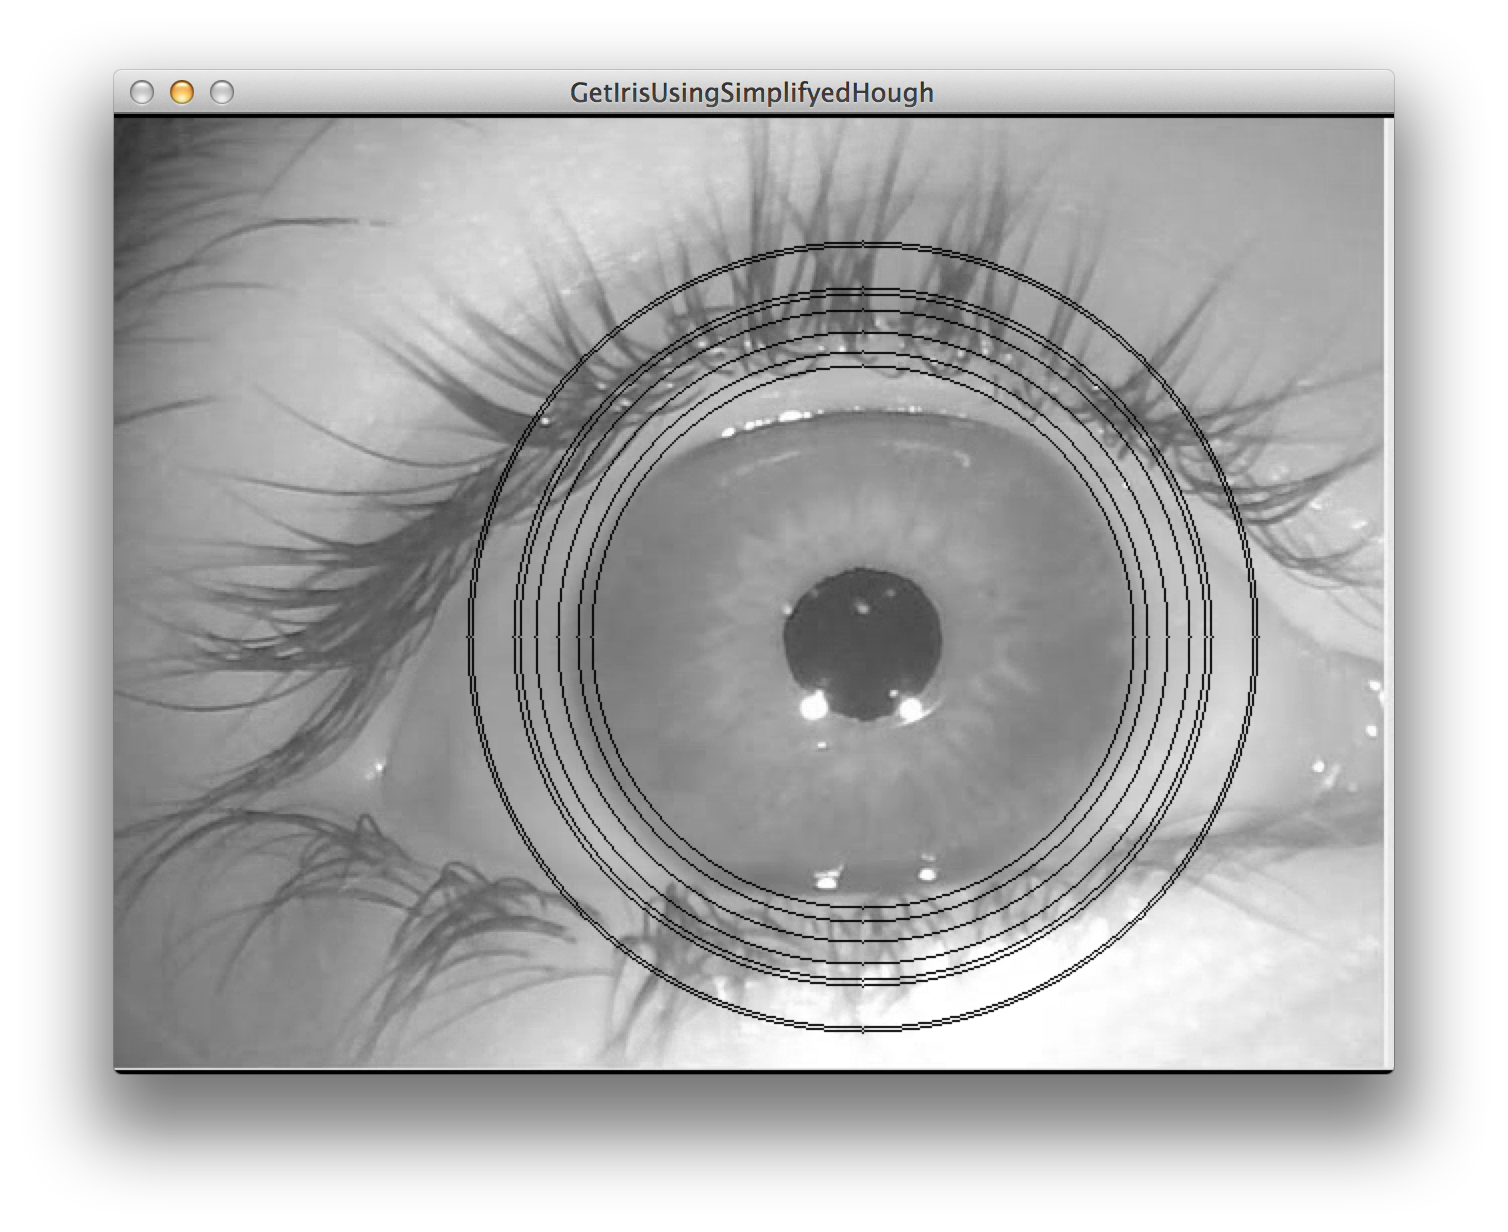
\includegraphics[width=.8\linewidth]{circhoughavg}
  \caption{One correct circle and some false positives}
  \label{fig:circhoughavg}
\end{subfigure}
\begin{subfigure}{.48\textwidth}
  \centering
  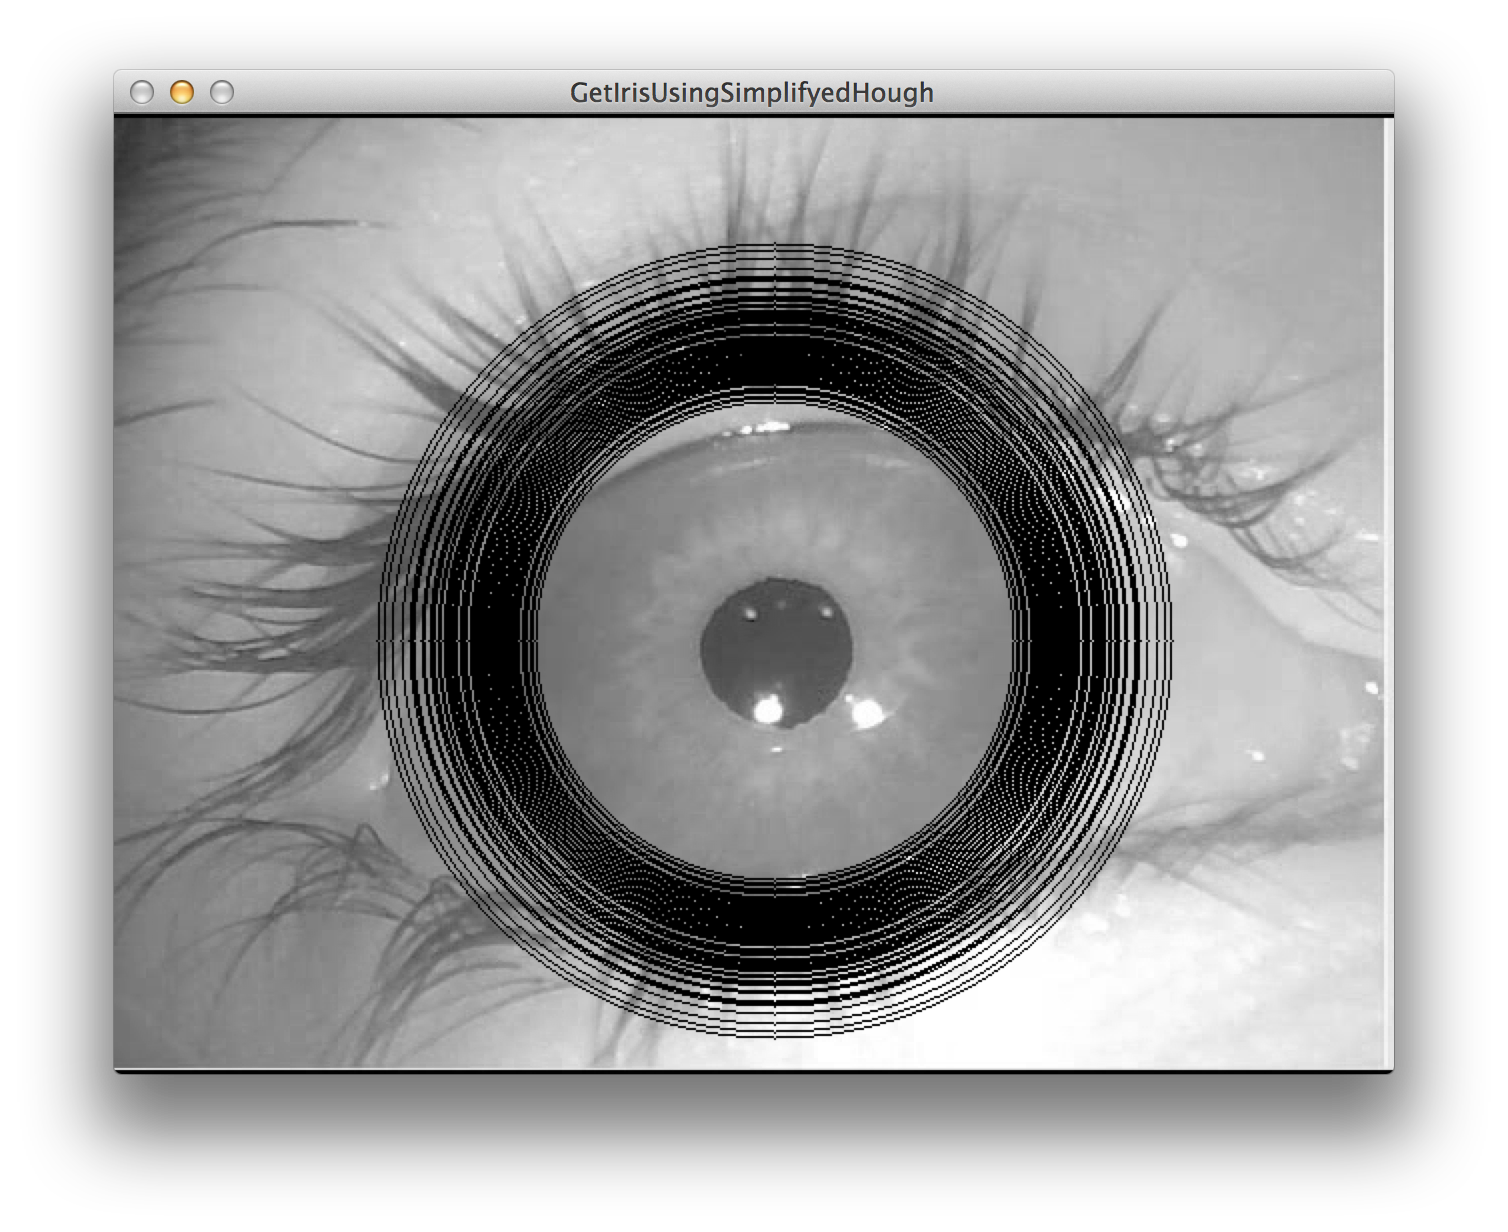
\includegraphics[width=.8\linewidth]{circhoughgood}
  \caption{Multiple true positives}
  \label{fig:circhoughgood}
\end{subfigure}
\caption{Detecting circles using Hough transformation with position prior }
\label{fig:houghcircles}
\end{figure}


\begin{figure}[H]
\centering
  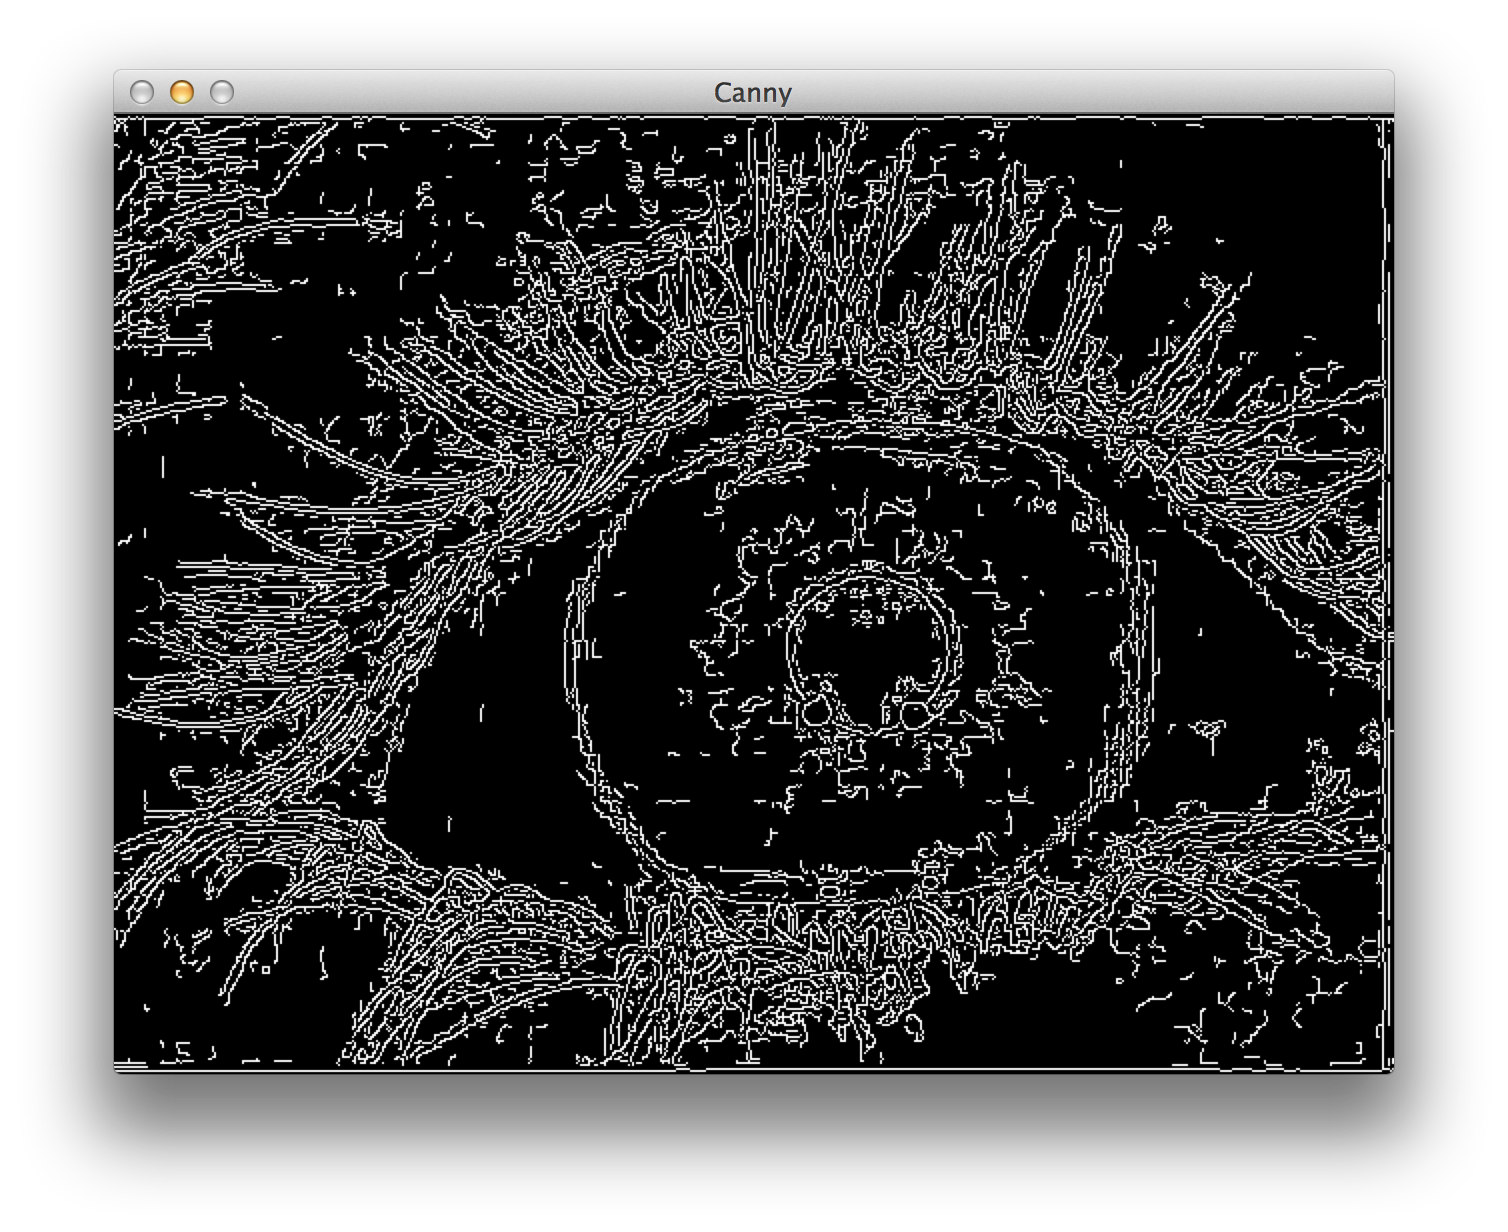
\includegraphics[width=.8\linewidth]{houghcanny}
  \caption{The canny edge image on which the circles in figure (a) are found}
  \label{fig:canny}
\end{figure}
In figure (a) the method positively identifies the limbus and some false positives.

In figure (b) the method yields more circles above some given threshold since the perspective distortion exhibits a limbus that appears to be more circular than it actually is.

\paragraph{Discussion} % (fold)
\label{par:discussion}
The method works but is sensitive on numerous parameters. The threshold should be carefully chosen, and is dependent on the granularity of the Canny edge image it takes as input. A canny edge image with a lot of edges yields an accumulator table with more votes, and thus more iris candidates.

Looking at Figure \ref{fig:canny} we see that one possible improvement could be to smoothe the image before producing the Canny edge image. This would remove the noise produced by eye lashes and other non-circular features.

\section{Conclusion}
After ample experimentation, we find that the following techniques perform best:
\paragraph{Pupil}
Hough transform gives a robust pupil detection, that works on image gradient, instead of actual intensity. This makes it much more tolerant of changing lighting conditions. We preprocess the input image with a Gaussian blur, to minimize the effect of noise.

\paragraph{Eye Corners}
We have only experimented with Template Matching for eye corner detection. We have not attempted to use a generic set of templates across multiple sequences, but have settled with having to define templates for each sequence.

\paragraph{Glints}
Our thresholding approach is extremely good at finding all the highlights of the image, but results in many false positives. Filtering those with blob detection eliminates most of the false positives. Further, requiring that the glints are close to the pupil center, results in a very robust glint detection (given that the pupil is correctly detected)

\paragraph{Iris / Limbus}
We use our own, simplified Hough transform, that assumes the pupil center has been found correctly, and that the limbus is approximately circular. This is the least robust of our feature detections, but works well enough in practice to be useful.

\begin{figure}[H]
  \centering
  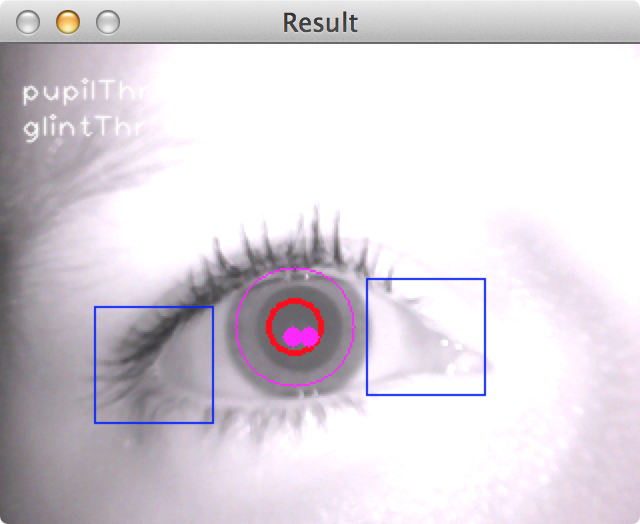
\includegraphics[scale=0.3]{resgood}
  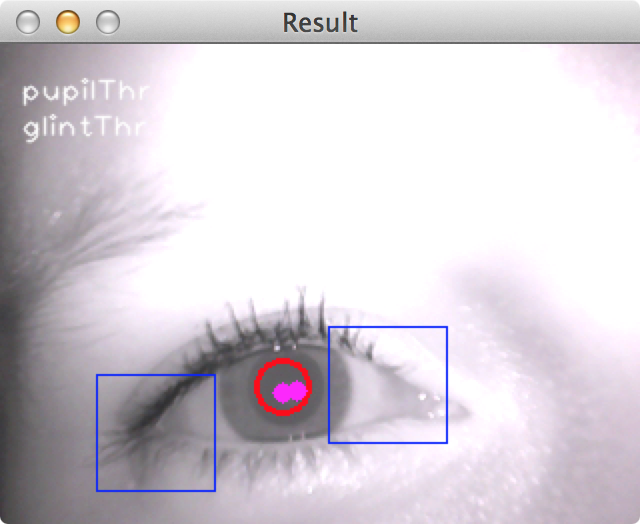
\includegraphics[scale=0.3]{resnoiris}
  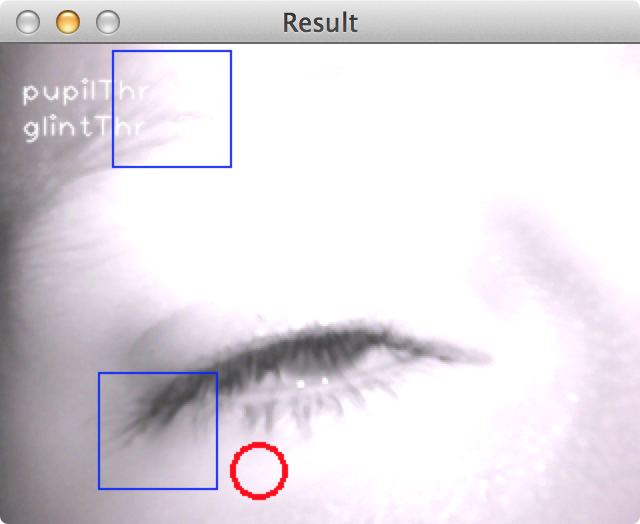
\includegraphics[scale=0.3]{resnotworking}
  \caption{Left: working detection, middle: Iris detection failed, right: Totally failed detection (blink)}
  \label{fig:results}
\end{figure}

\paragraph{Performance}
We have recorded our own sequence: 'Julie.avi', using an iSlim 321r camera with infrared capabilities. Figure \ref{fig:results} shows an image from 'Julie.avi' where detection is successful, and an image where the detection fails. Enclosed on the CD-ROM is the full sequence 'Julie.avi' (unedited recording), and 'Julie\_Detection.avi' that shows the performance of our eye tracker across the entire sequence. \\

There is certainly room for improvement, especially in the areas of eye corner and iris detection. But overall we are happy with the performance of our eye tracker, especially the various Hough transforms we apply, perform very well.
\newpage

\section*{Appendix}
\subsection{Assignment1.py}
\lstinputlisting[language=Python]{../ass1/Assignment1.py}


\end{document}
